
\documentclass[10pt,journal,compsoc]{IEEEtran}
%\documentclass[usemulticol,english]{cccconf}
\usepackage[comma,numbers,square,sort&compress]{natbib}
\usepackage{graphicx,times,amsmath}
\usepackage{graphicx}      % include this line if your document contains figures
\usepackage{natbib}        % required for bibliography
%\usepackage[comma,numbers,square,sort&compress]{natbib}
\usepackage{indentfirst}
\usepackage{mathbbold}
\usepackage{mathrsfs}
\usepackage{amsmath,amssymb}
\usepackage{amsfonts}
\usepackage{mathrsfs}
\usepackage{pifont}
\usepackage{bbding}
\usepackage{amssymb}
\usepackage[T1]{fontenc}
\usepackage{color}
\usepackage{units}
\usepackage{amsmath}
\usepackage{amssymb}
\usepackage{stackrel}
\usepackage{graphicx}
\usepackage{esint}
\usepackage{caption}
\usepackage{subcaption}
%\usepackage{subfigure}
\usepackage{enumerate}
%\usepackage{caption}
%\usepackage{subcaption}
\usepackage{dcolumn}
\usepackage{makecell}
\usepackage{booktabs}
\usepackage{algorithm}
\usepackage{algorithmic}

\makeatletter
\newcommand{\lyxdot}{.}
\newtheorem{remark}{Remark}
\newtheorem{thm}{Theorem}
\newtheorem{lem}{Lemma}
\newtheorem{suppose}{Suppose}
\newtheorem{proof}{Proof}
\newtheorem{asum}{Assumption}
\makeatother

\begin{document}
%
\title{Privacy preserving consensus under interception attacks}
\author{Wen~Yang,~\IEEEmembership{Member,~IEEE,}
        John~Doe,~\IEEEmembership{Fellow,~OSA,}
        and~Jane~Doe,~\IEEEmembership{Life~Fellow,~IEEE}% <-this % stops a space
\IEEEcompsocitemizethanks{\IEEEcompsocthanksitem M. Shell was with the Department
of Electrical and Computer Engineering, Georgia Institute of Technology, Atlanta,
GA, 30332.\protect\\
% note need leading \protect in front of \\ to get a newline within \thanks as
% \\ is fragile and will error, could use \hfil\break instead.
E-mail: see http://www.michaelshell.org/contact.html
\IEEEcompsocthanksitem J. Doe and J. Doe are with Anonymous University.}% <-this % stops an unwanted space
\thanks{Manuscript received April 19, 2005; revised August 26, 2015.}}

\markboth{Journal of \LaTeX\ Class Files,~Vol.~14, No.~8, August~2015}%
{Shell \MakeLowercase{\textit{et al.}}: Bare Demo of IEEEtran.cls for Computer Society Journals}

\IEEEtitleabstractindextext{%
\begin{abstract}
In this paper, we consider the attack problem in privacy-protected networks. First, we introduce a consensus protocol with privacy preserving, where each node hide their initial state into a set of random sequences, and then inject the sequences into the process of consensus. Due to the protocol will fail in the special network topology, we consider the situation where an attacker can intercept the data transmitted on the edges, and obtain an indicator which can measure the degree of privacy leakage. In ring and small-world networks, from the perspective of the attacker with limited power, we find the optimal attacking strategy to maximize the probability of the privacy disclosure. Finally, we provide an optimization algorithm to verify the results of the analysis, and we can use this algorithm to find the optimal attack strategy for any other networks.
\end{abstract}

% Note that keywords are not normally used for peerreview papers.
\begin{IEEEkeywords}
Privacy preserving; Consensus protocol; Interception attack
\end{IEEEkeywords}}


% make the title area
\maketitle


% To allow for easy dual compilation without having to reenter the
% abstract/keywords data, the \IEEEtitleabstractindextext text will
% not be used in maketitle, but will appear (i.e., to be "transported")
% here as \IEEEdisplaynontitleabstractindextext when the compsoc
% or transmag modes are not selected <OR> if conference mode is selected
% - because all conference papers position the abstract like regular
% papers do.
\IEEEdisplaynontitleabstractindextext
% \IEEEdisplaynontitleabstractindextext has no effect when using
% compsoc or transmag under a non-conference mode.



% For peer review papers, you can put extra information on the cover
% page as needed:
% \ifCLASSOPTIONpeerreview
% \begin{center} \bfseries EDICS Category: 3-BBND \end{center}
% \fi
%
% For peerreview papers, this IEEEtran command inserts a page break and
% creates the second title. It will be ignored for other modes.
\IEEEpeerreviewmaketitle



\section{Introduction}

As a typical distributed algorithm, consensus protocol has been widely used in many fields, including control engineering, computer science, system biology and physics, where each node exchanges information with its linked neighbors such that the whole network reaches an agreement. Consensus problem has attracted many researchers in recent decades, from protocol design, convergence analysis to network performance optimization, it has been studied extensively, see
 \cite{Olfatisaber2004Consensus,Olfati2007Consensus,Shi2012Optimal,yang2013fast,Yang2016Nodes}.

Recently, wireless security has received a lot of research attention. Privacy information leakage is one of the important topics. For example, a distributed network can achieves consensus when each node exchanges its state with it's neighboring nodes, at the same time, the initial states of all the nodes are broadcast to the whole network, see \cite{Mo2016Privacy}, \cite{Kolesnikov2009Advances}. In practical applications, such as decision-making scenes, how to keep the participant's information secrete is a key problem while achieving the goal of reaching the agreement. Therefore, many researchers focus on the privacy preserving problem. In \cite{Dwork2006Differential}, the author proposed the notation of differential privacy (DP), and gived a mathematical definition of privacy level. Huang applied the DP approach to the problem of consensus protocol, \cite{Huang2012Differentially} proposed a privacy protection protocol by adding independent and exponentially decaying Laplacian noise in the process of consensus updating. However, there is a problem with the protocol based on DP, which is unable to converge to the accurate mean of the initial state. Therefore, in some cases, the DP method can not be used. For maximum consensus, in \cite{Duan2015Privacy}, the authors devised a protocol to send a special offset before sending the actual initial state. For average consensus, Mo et al.\cite{Mo2016Privacy} proposed a privacy preserving algorithm by adding well-designed noise on its state, then the author analysis the convergence rate of this consensus algorithm, and prove the algorithm achieves minimum privacy breach. In \cite{Manitara2013Privacy}, the author presented a privacy preserving consensus algorithm that each node adds an arbitrary offset value to the result of iteration, where the total offsets cancel themselves out in the end. Moreover, in \cite{Mo2016Privacy, Manitara2013Privacy}, they all put restrictions on network structure, i.e., if a node and all of it's neighbors belong to the malicious node's neighboring node set, the node's initial state can be speculated by the malicious node.

Currently, plenty studies focus on cyber attacks that happen frequently in real applications, see \cite{Kefayati2007Secure,Zhang2014Online,Qi2015,Lei2016Fast}. However, less studies have been directed to the privacy preserving under malicious attacks. In recent years, complex network has been widely used to describe the system in nature. \cite{Watts1998Collective} proposed an interesting small-world network model, referred to as WS small-world model. Many profound studies are based on the small-world model, see \cite{Hong2002Synchronization,Wang2003Complex}. In \cite{XIAO2011SYNCHRONIZATION}, the author study how the structures of networks affect their synchronization, In this article,  we will use small-world network as one of our attack model.

In this paper, we first introduce an average consensus protocol with privacy preserving proposed in \cite{Manitara2013Privacy}, and point out one of its defects, when the network topology meet certain conditions, there will be leakage of privacy information. Once there is an attacker in the network, it can intercept the data transmitted on the edges, and then can deduce the initial state of the nodes in the network. If the attacker's energy is limited, we study the relationship between the degree of the private information leakage and the energy allocated on each edge. Specific to ring network and small-world networks, we try to find the optimal attacking strategy, resulting in the greatest degree of privacy leakage. The main contributions of this article are summarized as: 1) We get a specific mathematical formula that can calculate the degree of privacy leakage; 2) In the ring network and small-world model, we theoretically analyze how to allocate the attacker's energy, which can maximize the attack effect; 3) We provide an algorithm that can be used to find the optimal attack strategy in any network; 4) By the simulation, we obtain the relationship between the convergence step and the variance of the added noise.

\emph{Notation:} $\mathbb{R}^{n\times m}$ denotes the set of $n$ by $m$ matrices. $e_{i}$ denotes the $i$th canonical basis in $\mathbb{R}^{n}$ with a 1 in the $i$th entry and zeros elsewhere.

\section{Problem formulation}\label{Problem formulation}
In this paper, we model a sensor network as an undirected graph $G =(V,E)$ with the nodes $V = {1,2,...,n}$ being the sensors and the edges $E\subset V \times V$ representing the communication links. Denote the set of neighbors of node $i$ by $N(i)=\{j\in V:(i, j)\in E, j\neq i\}$. Each node can communicate with its neighbors. The interconnection topology of the network is described by Laplacian matrix $L=[l_{ij}]$, where $l_{ii}=-\sum_{j \in N_i}l_{ij}$ and $l_{ij}=-1$ if $(i, j) \in E$; otherwise, $l_{ij}=0$. Assume that $G$ is connected, and let the initial state of each node is $x_{i}(0)$. In the network, each node updates its state according to the following consensus protocol (see \cite{Olfatisaber2004Consensus}),
\begin{equation} \label{Update equation}
\begin{split}
x_{i}(k+1)&=x_{i}(k)+\varepsilon\underset{j\in N(i)}{\sum}a_{ij}(x_{j}(k)-x_{i}(k)).
\end{split}
\end{equation}
By collecting all the states of the nodes, we define $x(k) \triangleq [x_1(k),\ldots,x_n(k)]'$. The single node dynamics (\ref{Update equation}) can be represented as the following vector form
\begin{equation} \label{Simple Update Form}
\begin{split}
x(k+1)=P_{\varepsilon}x(k),
\end{split}
\end{equation}
where $P_{\varepsilon}=[a_{ij}]$ (called as \textit{Perron matrix}) is satisfied with
 \begin{equation} \label{Calculate P}
\begin{split}
P_{\varepsilon}=I-\varepsilon L.
\end{split}
\end{equation}
We denote the node with maximum number of neighbors of in $G$ as $d_{max}=max\{l_{ii}\}$, then $\varepsilon \in (0, 1/d_{max})$ is satisfied to guarantee the convergence of protocol (\ref{Simple Update Form}), see \cite{Olfatisaber2004Consensus}. Moreover, based on the existing results in \cite{Olfatisaber2004Consensus}, the node dynamics (\ref{Simple Update Form}) asymptotically solves the average consensus problem if and only if $G$ is balanced.

In this paper, we study the privacy preserving of consensus protocol under typical attacks. First, we assume that node $n$ wants to infer the initial states of all the other nodes in the network. We denote the neighboring set of node $n$ as $N(n)=\{j_{1},\ldots,j_{m}\}$, and define an observation matrix $C$ as
$
C=[e_{j_{1}},...,e_{j_{m}},e_{n}]^{T}\in \mathbb{R}^{(m+1)\times n},
$
The output equation of the whole network can be rewritten as the following,
\begin{equation}\label{Output equation}
\begin{split}
y(k)=Cx(k).
\end{split}
\end{equation}
At time step $k$, node $n$'s information set is
\begin{equation} \label{Information matix}
\begin{split}
I(k)=\{x_{n}(0), y(0), ...y(k)\}.
\end{split}
\end{equation}

\begin{lem}
(\cite{Mo2016Privacy})
Assume node $n$ knows $P_{\varepsilon}$ and $C$ matrices and all variables in $I(k)$ at time step $k$, the consensus algorithm is deterministic and node $n$ can perfectly infer $\zeta'x(0)$, given that $\zeta \in \mathbb{R}^{n}$ lies in the observable space of ($P_{\varepsilon}, C$).
\end{lem}
To protect the privacy of the initial states of nodes while enforce $x(k)$ converges to the average of $x(0)$, \cite{Manitara2013Privacy} proposes a consensus protocol with privacy preserving scheme in a weighted and directed network. In this paper, we focus on analyze the network performance of privacy preserving consensus protocol under a typical attack, and then simplify this privacy preserving scheme to the case when the network is unweighted and undirected.

The steps of {\bf privacy preserving scheme} are listed as follows:
\begin{enumerate}[1)]
\item Each node $i$ generates a random number $m_{i}$, which satisfied with $2\leq m_{i} \leq M$, $M$ is a positive real number.
\item Each node generates $m_{i}$ random number which are denoted as ${r_{i}(1), r_{i}(2), ..., r_{i}(m_i)}$, with their average value is $x_{i}(0)$.
\item Clear the initial state of each node to $x_{i}(0)=0$, we mark the real initial state as $x_{i}^{r}(0)$, thus we can define $x^{r}(0)=[x_{1}^{r}(0), x_{2}^{r}(0) ...x_{n}^{r}(0)]^{T}\in\mathbb{R}^{n}$.
\item At time step $k$, inject the number $d_{i}(k)$ into the state of each node, where
\[
d_{i}(k)=\begin{cases}
r_{i}(k)/m_i, & if\, 1\leq k\leq m_{i} \\
0, & otherwise.
\end{cases}
\]\\
\end{enumerate}
According to the above four steps, each node updates its state by
\begin{equation}\label{Eqn: node dynamics with privacy protection}
\begin{split}
x_{i}(k+1)&=x_{i}(k)+\varepsilon\underset{j\in N_{i}}{\sum}a_{ij}(x_{j}(k)-x_{i}(k))+d_{i}(k+1),
\end{split}
\end{equation}
Define $d(k)=[d_{1}(k), ...,d_{n}(k)]^{T}\in\mathbb{R}^{n}$. The vector form of (\ref{Eqn: node dynamics with privacy protection}) in conjunction with Eq. (\ref{Output equation}) can be rewritten as
\begin{equation}  \label{new update rule}
\begin{split}
\begin{cases}
x(k+1)=P_{\varepsilon}x(k)+d(k+1), \\
y(k)=Cx(k).
\end{cases}
\end{split}
\end{equation}

Based on the above scheme, the real initial states of nodes are hidden in several parts, thus the privacy of $x^r(0)$ can be protected.
\section{Main Result}\label{Main Result}

\subsection{Privacy Analysis}\label{subsection: Privacy Analysis}
With a standard consensus algorithm, the initial states of nodes can be easily speculated by any other nodes. However, with the proposed privacy preserving algorithm (\ref{Eqn: node dynamics with privacy protection}), all the nodes reach average consensus finally, and the real initial states of nodes are hidden in $d(k)$. Hence, the problem of deducting $x^{r}(0)$ actually can be transformed into computing $d(k), k\in [1, M]$. First, we obtain the solution of (\ref{new update rule}) by iterative method.
\begin{equation} \label{solution of update rule}
\begin{split}
x(k)=&P_{\varepsilon}^{k}x(0)+\sum_{i=0}^{k-1}P_{\varepsilon}^{k-1-i}d(i+1), \\
y(k)=&CP_{\varepsilon}^{k}x(0)+C\sum_{i=0}^{k-1}P_{\varepsilon}^{k-1-i}d(i+1).
\end{split}
\end{equation}
Recalling that $x(0)=0$, we obtain:
\begin{equation} \label{compute Y}
Y=FD
\end{equation}
where,
\[
F=\begin{bmatrix}
C & 0 & \dots & 0\\
CP_{\varepsilon} & C &\dots & 0\\
\vdots &\vdots &\ddots & \vdots\\
CP_{\varepsilon}^{M-1}&CP_{\varepsilon}^{M-2} & \dots & C
\end{bmatrix}\in\mathbb{R}^{((m+1)M)\times(nM)}
\]
\[Y=
\begin{bmatrix}
y(1)\\
y(2)\\
\vdots\\
y(M)
\end{bmatrix}, D=
\begin{bmatrix}
d(1)\\
d(2)\\
\vdots\\
d(M)
\end{bmatrix}\in \mathbb{R}^{nM\times1}.
\]

For a fixed network topology $G$, $F$ is a constant matrix. In order to derive the the real initial state $x^{r}(0)$ from $D$, we need to utilize the information $Y$ to solve the equation (\ref{compute Y}).
Let us define
\[
\begin{split}
s_{i}=\begin{cases}
e_{i}, &if\ i\in N(n) \\
\mathbf{0}, &else
\end{cases}
\end{split}
\]
where $\mathbf{0}\in \mathbb{R}^{n}$ is zero vector.
We further define:
\[
\begin{split}
\tilde{C}=&[s_{1}, s_{2}, ...s_{n}]^{T}\in\mathbb{R}^{n\times n},\\
\tilde{y}(k)&=\tilde{C}x(k)\in\mathbb{R}^{n\times 1},
\end{split}
\]
where $\tilde{y}(k)$ is easily obtained from $y(k)$ for a given $C$.

Using all the above arguments, we obtain the following result.
\begin{thm}
If the $i$th line of $P_{\varepsilon}$ noted as $P_{\varepsilon_i}$ satisfies $P_{\varepsilon_i}\tilde{C}=P_{\varepsilon_i}$, then node $n$ can speculate the initial state of node $i$ successfully.
\end{thm}

\begin{proof}
For any $k\in[1, M-1]$, we have
\[\tilde{y}(k)=\tilde{C}\sum_{i=0}^{k-1}P_{\varepsilon}^{k-1-i}d(i+1).\]
Note that $P_{\varepsilon_i}\tilde{C}=P_{\varepsilon_i}$. We know that node $i$ is one neighbor of node $n$, thus $x_{i}(k)$ lies in the $i$th line of $y(k)$, then
\begin{equation}
\begin{split}
P_{\varepsilon_i}\tilde{y}(k)&=P_{\varepsilon_i}\sum_{i=0}^{k-1}P_{\varepsilon}^{k-1-i}d(i+1)\\
&=P_{\varepsilon_i}x_{i}(k).
\end{split}
\end{equation}
At time step $k+1$, we can derive $x_{i}(k+1)$ from $y(k+1)$. Hence,
\begin{equation}
d_{i}(k+1)=x_{i}(k+1)-P_{\varepsilon_i}x_{i}(k).
\end{equation}
By this way, we can also obtain $(d_{i}(2), d_{i}(3)...d_{i}(M)$. Note that $d_{i}(1)$ lies in $y(1)=Cd(1)$. Finally, we can obtain the initial state of node $i$. Thus the proof. $\blacksquare$
\end{proof}

As mentioned above, there still exists the possibility that node $i$'s initial state can be speculated under a special structure of network $N(i)\bigcup{i}\subseteq N(n)\bigcup{n}$. If there exists an attacker who can intercept the information flow between pairs of nodes, then the initial states of parts of nodes could be deducted. Therefore, the performance of privacy preserving drops greatly. On the other hand, the attacker is usually equipped with limited power, which implies that it needs to allocate the power to launch an attack reasonably according a certain scheme. To design effective strategies to defend against the attacks, it is necessary to study the attacking way of the attacker. In the following, we try to find an optimal attacking strategy from the perspective of the attack, and then in turn help us design strategy to preserve the privacy better.


\subsection{Attack Analysis}\label{subsection: attack analysis}
In this subsection, we consider the case when an attacker with limited power exists in the network. Suppose that the probability of the attacker intercepting the information transmitted on the edge between node $i$ and node $j$ as $\lambda_{i, j}$. Recall that the network is undirected, it's unnecessary to distinguish $\lambda_{i, j}$ and $\lambda_{j, i}$, i.e., $\lambda_{i,j}=\lambda_{j,i}$. To make the statement more clearly, we use $g_{i, j}$ to represent the edge in the network, where $g_{i,j}$ and $g_{j,i}$ represent the same edge. We assume that $\lambda_{i, j}$ depends on the power $\mu_{i, j}$ allocated for the attack on the edge $g_{i, j}$, where $\lambda_{i, j}=\kappa \cdot \mu_{i, j}$. Define the power constraint of the attacker as $\sum_{g_{i,j}\in E}\mu_{i, j}=T$, for all $i, j=1,\ldots,n$. Here, we set $\kappa=\frac{1}{T}$, and then $\sum_{g_{i,j}\in E}\lambda_{i, j}=1$.

As discussed above, we know that the privacy of node $i$ will be exposed in some situations. In Fig. (\ref{fig1}), let $i=1$.

\begin{figure}[!htb] \label{wireless network}
 \centering
 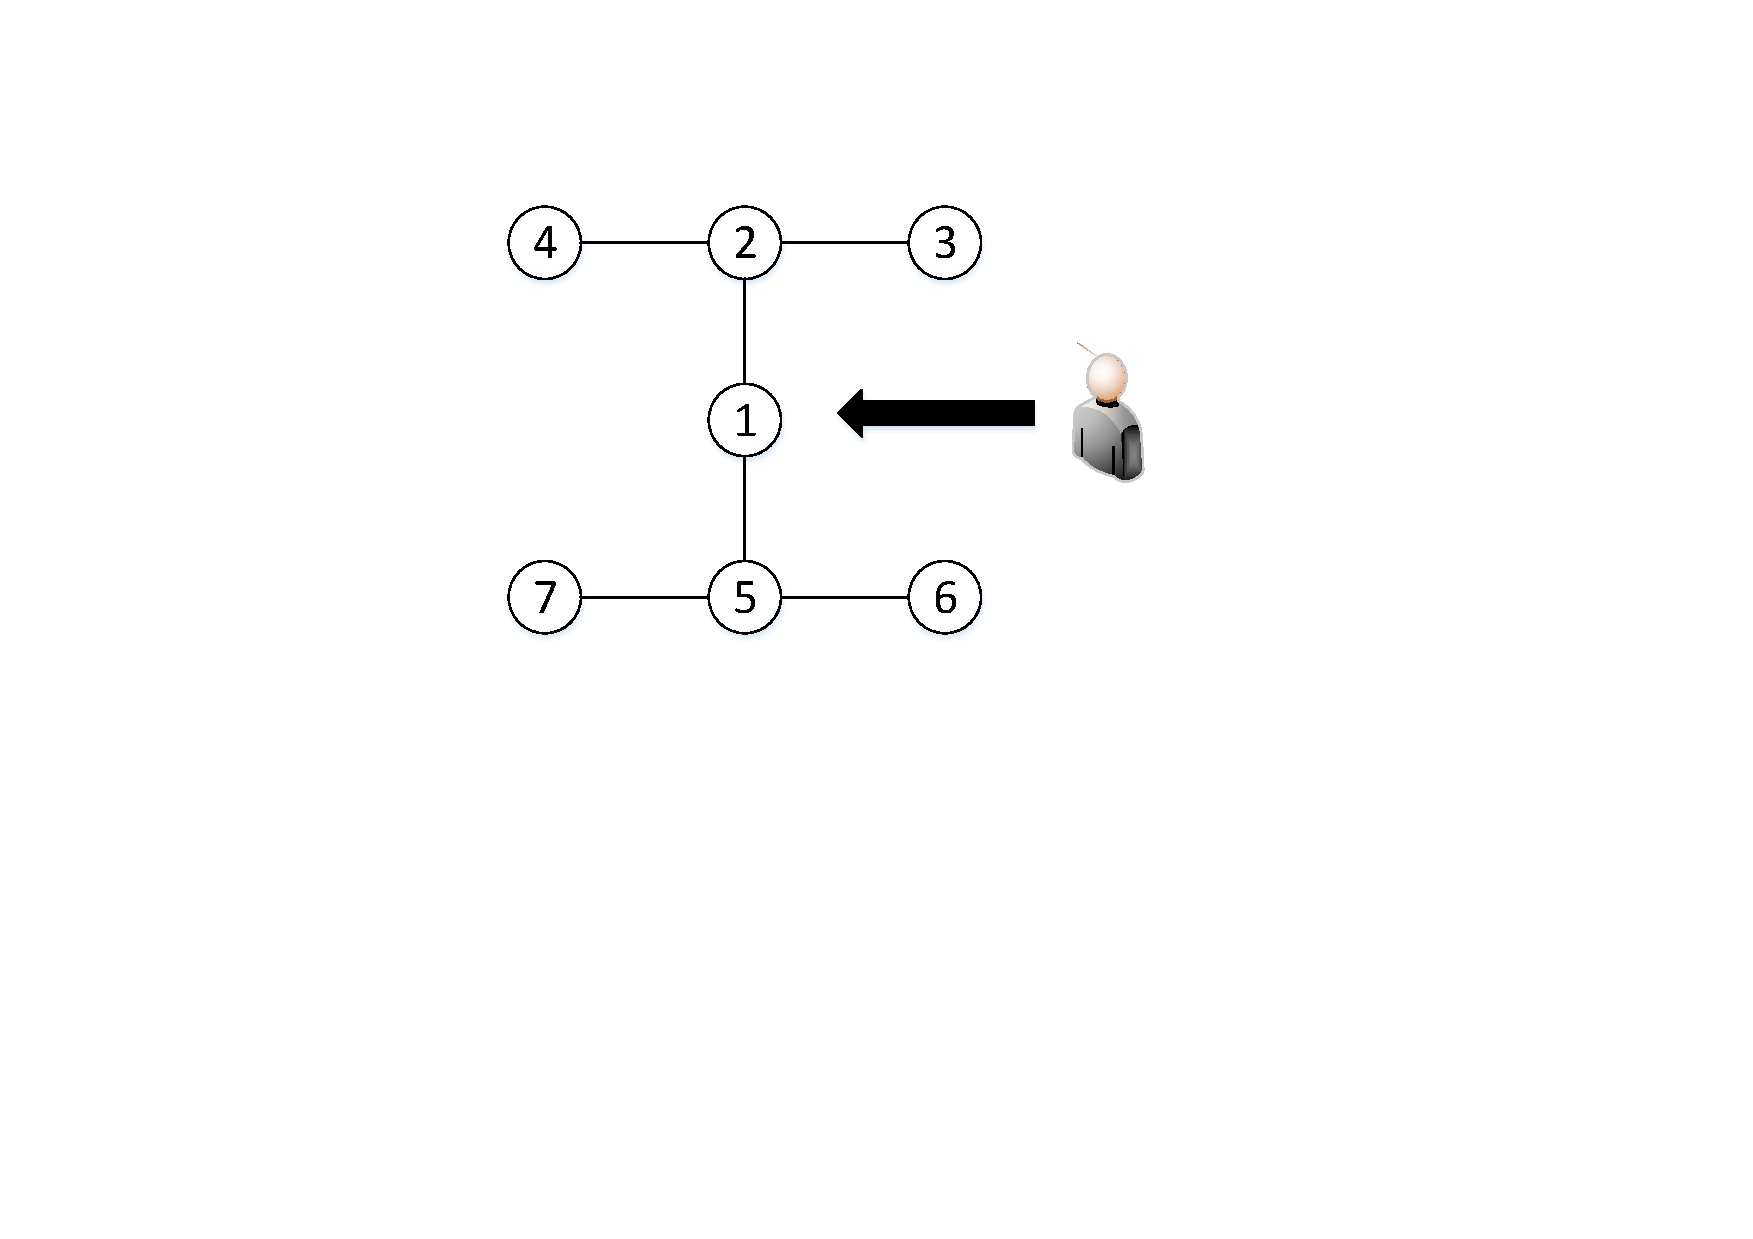
\includegraphics[width=5cm, height=3.2cm]{AttackNetwork}
 \caption{wireless network}
 \label{fig1}
\end{figure}

\begin{enumerate}[1)]
\item When the information passed on edge $g_{1, 2}$ and $g_{1, 5}$ have been exposed, at time step $k$, the attacker can easily utilize the obtained knowledge to predict the state of node $1$ at time step $k+1$ as $\hat{x}_{1, k+1}$, which does not contain the offset $d_{1}(k+1)$.  According to the information transmitted from node $1$ to node $5$ at time step $k+1$, $x_{1, k+1}$, we can further obtain the injected value which equals to$x_{1, k+1}-\hat{x}_{1, k+1}$. The attacker can derive the injection value of each step, then the initial state of node $1$ will be exposed.
\item When the information passed on the edge $g_{1, 2}$ and $g_{5, 6}$ have been exposed, at time step $k$, because of the information sent from node $5$ to it's neighbors are identical, the attacker can speculate all the messages sent to node $1$, then it can complete the speculating mission in the similar way.p
\end{enumerate}

As discussed above, once the network is under the situation similar to the case 2), then the privacy of the states will be divulged. For example, the information flow of edge $g_{1, 5}$ and $g_{2, 4}$'s is exposed.
\begin{remark}\label{exposed condition}
Suppose that there exists an attacker who can attack the network. If at least the information of one edge $g_{i,j}, j\in{N_i}$ has been intercept, and for each node $j, j\in N_i$, at least the information of one edge $g_{j,s}, s\in{N_j}$ has been exposed, then the attacker can infer the initial state of node $i$ successfully.p
\end{remark}
In the following, we further consider the privacy preserving problem when the network is under attacks.  In a random network, we choose an edge to attack with identical power at each time step, i.e., the information transmitted on the chosen edge is intercepted by the attacker successfully. In the case when the allocated power is zero, we regard the edge does not suffer any attack. Then we denote the adjacency matrix of the attacked network as $A_d$, $A_d[i, j]=1$ represents a connected edge between node $i$ and $j$, then we can define the attacking matrix $A_t$, which satisfies
\[
A_t[i, j]=\begin{cases}
\lambda_{i, j}, & if \ A_d[i, j]=1 \\
0, & otherwise,
\end{cases}
\]\\
Notice $\lambda_{i, j}=\lambda_{j, i}$, so $A_t=A_t^T$.

To investigate the influence of the attacker on the privacy preserving, we define $P_i$ as the probability of privacy leakage of node $i$, $i=1,2,\ldots,n$, i.e., the probability
of the attacker deducts the initial state of node $i$ successfully.
\begin{thm}\label{Them of leakage possibility}
When the network is attacked by an attacker who can intercept the information transmitted on the edge, the probability of privacy leakage of node $i$, $i=1,2,\ldots,n$ can be calculated as,
\begin{equation}
\begin{split} \label{leakage possibility}
P_i&=W_{i}-W_{i}^{'}, \\
W_{i}&=\prod_{m\in N(i)}[1-\prod_{t=1}^{n}(1-e_{t}^{T}A_{t}e_m)], \\
W_{i}^{'}&=\prod_{m\in N(i)}[1-\prod_{t=1, t\neq i}^{n}(1-e_{t}^{T}A_{t}e_m)]
\end{split}
\end{equation}
\end{thm}
\begin{proof}
Note that $A_t(i, j)$ denotes the probability of edge between $i$ and $j$ attacked, actually, which equals to $e_i^{T}A_{t}e_{j}$. According to Remark (\ref{exposed condition}), if at least of one element at the $i$'s line in $A_d$ does not equal to zero, it means that at least one edge exists.

The probability of at least one edge connected to node $m$ is intercepted equals to $1-\prod_{t=1}^{n}(1-e_{t}^{T}A_{t}e_m)$, and the probability of at least one edge between $m$ and it's neighbors except node $i$ exposed equals to $1-\prod_{t=1, t\neq i}^{n}(1-e_{t}^{T}A_{t}e_m)$. Thus, $W_{i}$ and $W_{i}^{'}$, the former represents that each node in $N(i)$ has at least one leaked edge, and similarly, $W_{t}^{'}$ has a quite similar format with $W_{t}$, but it is worth noticing that in $W_{t}^{'}$ only considers the neighboring node's edge except $g_{i, m}$. Finally, the gap between $W_{i}$ and $W_{i}^{'}$ equals to the probability of the leakage of node $i$'s initial state. $\blacksquare$
\end{proof}

We denote the degree of the network's privacy being exposed as $P=\sum_{i=1}^{n}P_i$. If there exists an attacker with limited power, we are interested in finding the optimal attacking strategy of the attacker resulting in the maximal $P$, and then protect the network security more effectively. In the network, there are some edges who are prone to privacy leaks when compared with the other edges, in the following, we formulate an optimization problem to find those edges in two typical networks, i.e., ring network and small world network.
\begin{equation} \label{Optimal_problem}
\begin{split}
(P_0):~~~~~&\max_{A_t}{P}\\
s.t. &\sum_{g_{i,j}\in E}\lambda_{i, j}=1 \\
&0\leq \lambda_{i,j}\leq 1
\end{split}
\end{equation}

\begin{enumerate}
\item \textbf{Case 1: ring topology (see Fig. \ref{fig2})}
\end{enumerate}
\begin{figure}[!htb]
 \centering
 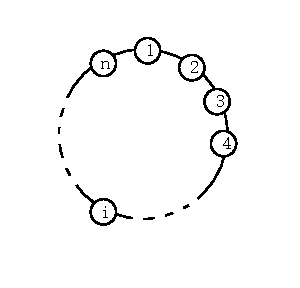
\includegraphics[width=4cm, height=4cm]{ring}
 \caption{Ring network}
 \label{fig2}
\end{figure}
In the ring network, the position of each node is identical. According to Theorem \ref{Them of leakage possibility}, we derive $P_{i}$ as follows:
\begin{equation} \label{Speculate P}
\begin{split}
P_i&=W_{i}-W_{i}^{'}\\
W_{i}&= H_{i-2}\cdot H_{i}\\
H_{i}&=1-(1-\lambda_{i, i+1})(1-\lambda_{i+1, i+2})\\
W_{i}^{'}&=\lambda_{i-2, i-1}\cdot(1-\lambda_{i-1, i})\cdot(1-\lambda_{i, i+1})\cdot\lambda_{i+1, i+2}
\end{split}
\end{equation}
The equation (\ref{Speculate P}) can be rewritten as
\begin{equation}
\begin{split}
P_i&=\lambda_{i-1, i}\cdot\lambda_{i, i+1}+\lambda_{i-1, i}\cdot\lambda_{i+1, i+2}+\lambda_{i-2, i-1}\cdot\lambda_{i, i+1}\\
&-\lambda_{i-2, i-1}\cdot\lambda_{i-1, i}\cdot\lambda_{i, i+1}-\lambda_{i-1, i}\cdot\lambda_{i, i+1}\cdot\lambda_{i+1, i+2}
\end{split}
\end{equation}

In order to simplify the notation, we use $\lambda_{i}$ to replace $\lambda_{i, i+1}$, particularly, $\lambda_{n}$ represents $\lambda_{n, 1}$. Due to the special structure of ring network, we can calculate $P$ by,
\begin{equation} \label{calculate P in ring network}
\begin{split}
P &= P_{1}+P_{2}+P_{3}...+P_{n}\\
&=\sum_{i=1}^{n}\lambda_{i}\cdot\lambda_{i+1}+2\sum_{i=1}^{n}\lambda_{i}\cdot\lambda_{i+2}-2\sum_{i=1}^{n}\lambda_{i}\cdot\lambda_{i+1}\cdot\lambda_{i+2}
\end{split}
\end{equation}
Here, we consider two cases,
\begin{enumerate}
\item when the attacker only attacks two edges, it means only two variables in $\lambda_{1},\lambda_{2},...\lambda_{n}$ are not equal to zero. The attacker has many choices, for example, it can attack two edges which connect to a same node, so that $\lambda_{i}$ and $\lambda_{i+1}$ are not zero, we can obtain the degree of the network's privacy being exposed $P = \lambda_{i}\cdot\lambda_{i+1}$, the constraint as $\lambda_{i}+\lambda_{i+1} = 1$. The attacker can also choose two edges who have the same neighboring edge, where $\lambda_{i}$ and $\lambda_{i+2}$ are not zero, we can calculate $P = 2\lambda_{i}\cdot\lambda_{i+2}$ with the constraint as $\lambda_{i}+\lambda_{i+2}=1$. Besides the above two cases, the attacker can also choose two edges that they don't connect to each other, and they also don't have any same neighboring edge, where $\lambda_{i}$ and $\lambda_{i+k}$ are not zero, $k \in {(2,n-2)}$, in these cases, we can obtain $P = 0$. According to all the above arguments, it is easy to derive the optimal attacking strategy corresponding to $\lambda_{i} = \lambda_{i+2}=0.5$, and the maximum $P = 0.5$.

\item when the attacker choose three edges, we can find the optimal attacking strategy using the similar above deductive method. When the attacker choose three edges to let $\lambda_{i},\lambda_{i+1},\lambda_{i+2}$ are not zero, we can obtain $P = \lambda_{i}\cdot\lambda_{i+1}+\lambda_{i+1}\cdot\lambda_{i+2}+2\lambda_{i}\cdot\lambda_{i+2}-2\lambda_{i}\cdot\lambda_{i+1}\cdot\lambda_{i+2}$ and the constraint is $\lambda_{i}+\lambda_{i+1}+\lambda_{i+2} = 1$.
Obviously, the index of $i$ will not influence the optimal value of $P$, without loss of generality, we let $i=1$ to simplify the notation. The optimization problem (\ref{Optimal_problem}) in this case can be rewritten as:p
\begin{equation}
\begin{split}
\max_{\lambda_{1},\lambda_{2},\lambda_{3}}\lambda_{1}\cdot\lambda_{2}+&\lambda_{2}\cdot\lambda_{3}+2\lambda_{1}\cdot\lambda_{3}-2\lambda_{1}\cdot\lambda_{2}\cdot\lambda_{3}\\
s.t. &0\leq\lambda_{1},\lambda_{2},\lambda_{3}\leq1 \\
&\lambda_{1}+\lambda_{2}+\lambda_{3} = 1 \\
\end{split}
\end{equation}
In this paper, we use Kuhn-Tucker Conditions to solve the above problem, the inequality constraint can be noted as $h_{i}(\lambda)\leq0$, $i\in[1,6]$,
\[
\begin{split}
h_{1}(\lambda) &= -\lambda_{1}\leq0\\
h_{2}(\lambda) &= \lambda_{1}-1\leq0\\
h_{3}(\lambda) &= -\lambda_{2}\leq0\\
h_{4}(\lambda) &= \lambda_{2}-1\leq0\\
h_{5}(\lambda) &= -\lambda_{3}\leq0\\
h_{6}(\lambda) &= \lambda_{3}-1\leq0
\end{split}
\]
The equality condition can be noted as $\Phi(\lambda) = \lambda_{1}+\lambda_{2}+\lambda_{3}-1 = 0$, and we use $\Gamma$ to denote the optimization function. Then
\[
\begin{split}
\nabla{\Gamma(\lambda)}+\sum_{i=1}^{6}\zeta_{i}\nabla{h_{i}(\lambda)}&+\psi\Phi(\lambda)=0 \\
\zeta_{i}h_{i}(\lambda) &= 0 \\
\Phi(\lambda) &= 0
\end{split}
\]
Finally, we can get the result as $\lambda_{1} = \lambda_{3}=0.5,\lambda_{2}=0$ and $P = 0.5$. When the chosen three edges satisfy that two edges are connect to each other, and the third one has a same neighbor with the first or second edge, where $\lambda_{i},\lambda_{i+1},\lambda_{i+3}\neq0$, we can obtain $P = \lambda_{i}\cdot\lambda_{i+1}+2\lambda_{i}\cdot\lambda_{i+2}$, and $\lambda_{i}+\lambda_{i+1}+\lambda_{i+3}=1$, when we let $i=1$, the optimal strategy is $\lambda_{2}=\lambda_{4}=0.5$, and $P=0.5$. When the chosen three edges are not direct connect to each other, but each of them has a common neighbor with another edge, where $\lambda_{i},\lambda_{i+2},\lambda_{i+4}\neq0$, and $\lambda_{i}+\lambda_{i+2}+\lambda_{i+4}=1$, we can calculate $P = 2\lambda_{i}\cdot\lambda_{i+2}+2\lambda_{i+2}\cdot\lambda_{i+4}$, when $i=1$, the optimal strategy is $\lambda_{3}=0.5,\lambda_{1}+\lambda_{5}=0.5$, and $P=0.5$. Once there is an chosen edge don't have common neighbor with others, we know that the allocation of this edge on this edge is a waste, so the analysis can be transformed into attacking on two edges. By the analysis, we can conclude that when the attacker choose three edges, the optimal strategy is $\lambda_{i+2}=0.5,\lambda_{i}+\lambda_{i+4}=0.5$, and $P=0.5$.
\end{enumerate}

The above analysis are based on the attacker allocated its energy to two or three edges. If the attacker can arbitrarily allocated its energy to any number of edges, we want to find the most destructive attack strategy. To solve this problem, We use the SLSQP (Sequential Least Squares Programming optimization algorithm) algorithm proposed in \cite{Kraft1994Algorithm}. Since the optimization algorithm may fall into the local optimum, the search result will depend on the position of the starting point, we search from the different starting positions separately to ensure that the optimal solution is as close as possible to the global optimization solution. The algorithm flow is as follows:
\begin{algorithm}[h]
\caption{\emph{Optimization algorithm}}
\begin{enumerate}[1)]
\item Generate the network topology to be analyzed.
\item Each non-zero element in $A_t$ is treated as a variable $v_{i}\in[0,1]$, and denote $V = [v_{1},v_{2},...v_{n}]$.
\item Write down the relationship between the extent of privacy leakage $P$ and each variable, and use $P_{optimal}=0$, $V_{optimal}=[0,0,...0]$ to save the final optimization results.
\item In the $k$th search, set the initial value of each variable as $V_{0}$. Then use SLSQP algorithm to find the optimal result, if the result is found successfully, we denote the maximum $P$ as $P_{optimal}(k)$, and the corresponding $V$ is $V_{optimal}(k)$. If $P_{optimal}(k)>P_{optimal}$, then we update $P_{optimal}$ and $V_{optimal}$ with $P_{optimal}(k)$ and $P_{optimal}(k)$.\label{repeat}
\item If $k+1 < 1000$, then generate a new initial set $V_{0}(k+1)$, and repeat the (\ref{repeat}) step, or end the optimization process.
\end{enumerate}
Where $V_{0}(k)$ is generated as follows:
\begin{enumerate}[1)]
\item Randomly select some variables from $V$, and the number of variables selected is random.
\item The selected variable assigns a random value between $[0,1]$.
\end{enumerate}
\end{algorithm}

For the 100-edge ring network, through the above optimization algorithm, we find the maximum $P = 0.5$, and the optimal strategy satisfied $\lambda_{i+2}=0.5,\lambda_{i}+\lambda_{i+4}=0.5$. The conclusion have some implications, for example, we can implement a special protection strategy for such structure, so as to protect the network security.

\begin{enumerate}[2)]
\item \textbf{Case 2: small-world topology (see Fig. \ref{figSW1},\ref{figSW2})}
\end{enumerate}

Using this optimization algorithm, we can not only study the ring network, but also other random network topology, Then the simulation results can be used to verify the theoretical analysis.

According to the results in Remark \ref{exposed condition}, for a general network topology under privacy protection, if the attacker want to get the initial state of node $i$, it should guarantee that at least the information of one edge connected to node $j$ has been exposed,$j\in N_i$, and at least the information of one edge connected to node $i$ has been intercepted, then the attacker can infer the initial state of node $i$ successfully.

If the attacker has limited energy, satisfied  $\sum_{g_{i,j}\in E}\lambda_{i, j}=1$, $\lambda_{i,j}$ is the probability of acquiring the channel information between $i$ and $j$. Though the rational allocation of the energy, the attacker can make the damage to the maximum, i.e., to maximize the degree of access to the network's private information.

By the result in Remark \ref{exposed condition}, obviously, if there is a node in the network with degree equal to 1, ie, there is only one edge connected to this node. It's only edge is the only channel for the node to communicate with the outside world, as long as this channel is eavesdropped, the attacker can perfectly infer the initial state of this node. For other nodes with degree grater than 1, the attacker should eavesdrop on the information in multiple channels, then the difficulty of attack will increase and the effect will be worse. Therefore, when there is a node with degree equal to 1, attacking the edge of this node is the best strategy. In the following, this inference is confirmed by simulation of small-world model.
\begin{figure}[!htb]
 \parbox[b]{.25\textwidth}{\centering
 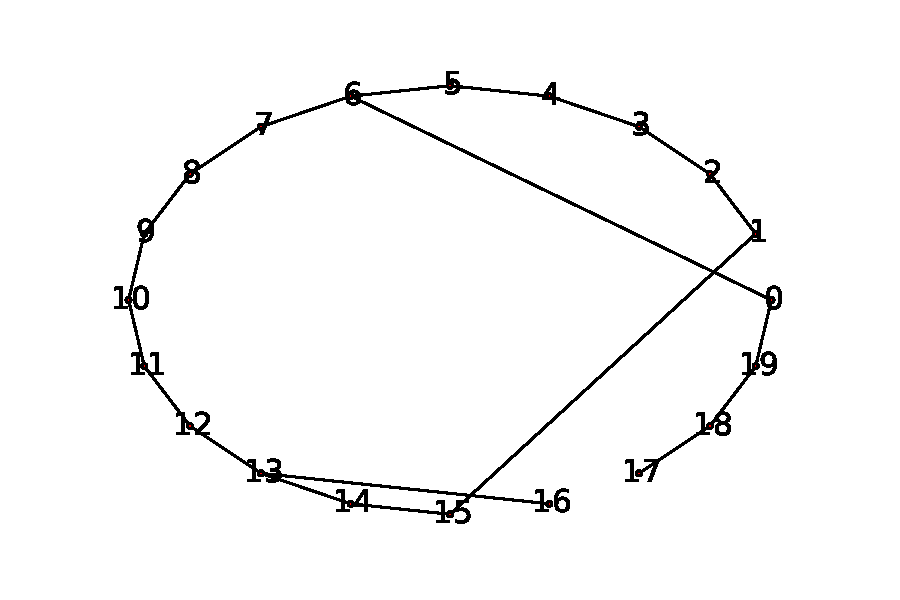
\includegraphics[width=4.2cm, height = 3.1cm]{k2p1-a}
 \subcaption{}\label{SW1-a}}%
 \parbox[b]{.25\textwidth}{\centering
 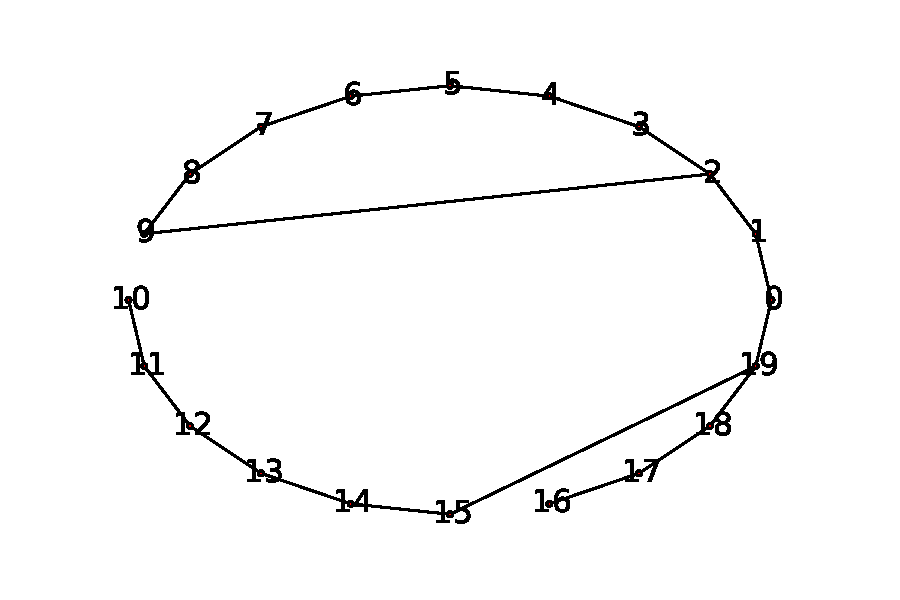
\includegraphics[width=4.2cm, height= 3.1cm]{k2p1-b}
 \subcaption{}\label{SW1-b}}
 \caption{Small World model 1}
 \label{figSW1}
\end{figure}

As we all know, The small-world Model is generated by a special regular network, and the generation rule is to cut some edges and randomly reconnect with other nodes with a certain probability. There are three indicators in the small-world model: the number of nodes $N$, the number of initial edges of each node $K$, the probability of reconnection $P_{reconnect}$. In Fig. \ref{figSW1}, two small-world model both are generated under condition $N=20,K=2,P_{reconnect}=0.1$. Using the optimization algorithm proposed earlier, we can find the optimal attack strategy in these network. In Fig. \ref{SW1-a}, the optimal result given by algorithm is $P=1$, the strategy satisfied $\lambda_{13,16}+\lambda_{17,18}=1$, notice where $\lambda_{i, j}$ represent the probability of the attacker intercepting the information transmitted on the edge between node $i$ and node $j$. In Fig. \ref{SW1-b}, the optimal result given by algorithm is $P=1$, the strategy satisfied $\lambda_{10,11}+\lambda_{16,17}=1$.

From the simulation result in Fig. \ref{figSW1}, we can see that the attack on the edge of the node which's degree equals to $1$ can bring the best attack effect, resulting in the greatest degree of privacy leakage. It should be noted that since the degree of leakage of the entire network is defined as the sum of the probabilities of private leaks of each node, the energy can be randomly assigned to all edges satisfying the condition. For example, In Fig. \ref{SW1-a}, the degree of node $16$ and node $17$ is 1, when the probability of obtaining the information on the unique edge of node $16$ is $\lambda_{13,16}$, by theorem \ref{Them of leakage possibility}, we can calculate $P_{16}=\lambda_{13,16}$, so the $P=P_{16}+P_{17}=\lambda_{13,16}+\lambda_{17,18}=1$.

 In real life, this phenomenon is easy to explain. In a social network composed of a number of participants, each participant has unique information, if such a network use the privacy protection strategy in this article, that is, each participant divide the information into several parts and then transmitted, to ensure the privacy of themselves. If a participant has only one channel communicating with the outside world, the eavesdropper can fully monitor the dynamics of the participant as long as he can get information flowing through the channel. For other participants with multiple information exchange channels, it is necessary to monitor multiple channels at the same time in order to achieve the purpose of obtaining the  initial information of the participant, at the same time, the cost of eavesdropping must be increased. So when the initial information of each participant is equally important, the eavesdropper is certainly more willing to eavesdrop on those participants who have only single information channel.

 When there is no degree 1 node in the network, the attacker will go looking for nodes whose degree is relatively small, to attack its edges or its neighbor's edges. By the result in Remark \ref{exposed condition}, we know that when we want to attack node $i$, i.e., to obtain the initial state of node $i$, the attacker can not only attack $i$'s edges directly, but also can eavesdrop $i$'s neighbor node's edges to get some important information. So there will be a very interesting situation, that is, when $i$'s neighbors are connected to each other, they share some information channel. When the attacker obtain the information passed by such channel, which is equivalent to obtaining the edge information of two node $j$, where $j\in N_{i}$. Then, we use small-world model to validate these analyzes.
\begin{figure}[!htb]
 \parbox[b]{.25\textwidth}{\centering
 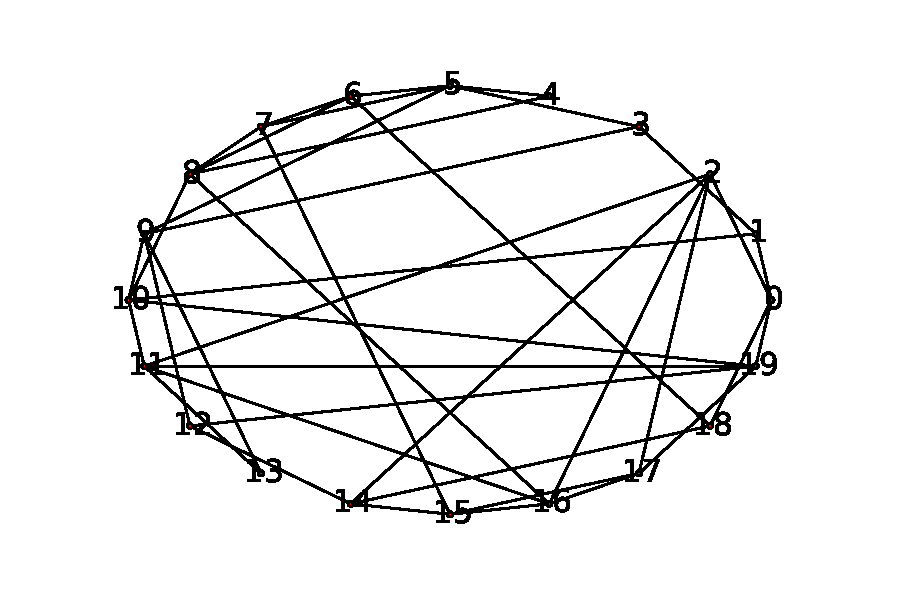
\includegraphics[width=4.2cm, height = 3.1cm]{k4p5-a}
 \subcaption{}\label{SW2-a}}%
 \parbox[b]{.25\textwidth}{\centering
 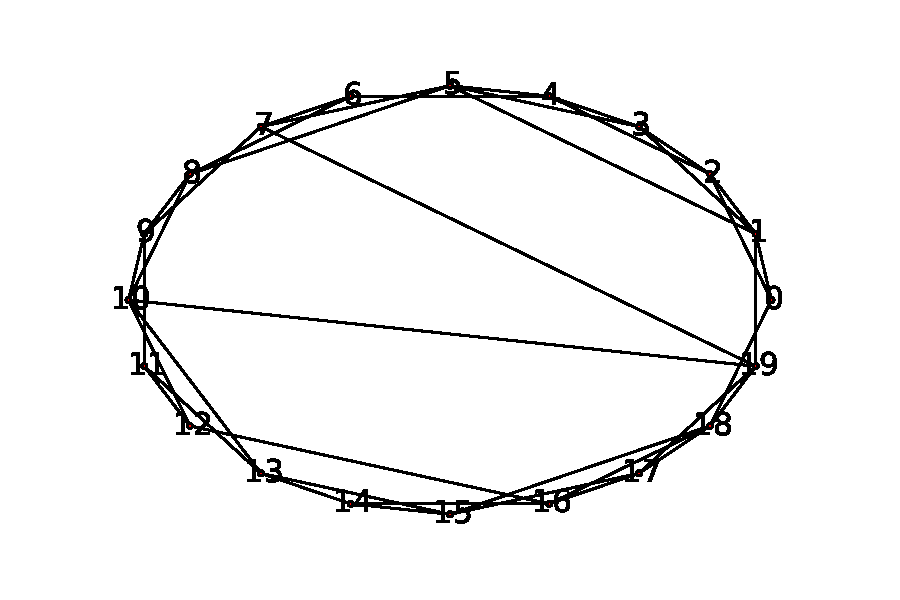
\includegraphics[width=4.2cm, height= 3.1cm]{k4p2}
 \subcaption{}}
 \caption{Small World model 2}
 \label{figSW2}
\end{figure}

In Fig. \ref{figSW2}, Fig. \ref{SW2-a} is generated under condition $N=20,K=4,P_{reconnect}=0.2$, the optimal attack strategy given by the algorithm is $\lambda_{4,5}=0.5,\lambda_{4,8}=0.5$, and the optimal result is $P=0.25$. By analyzing the network topology in Fig. \ref{SW2-a}, we can find that the $4$ is the only node with degree equals to 2, and the degree of other nodes is greater than or equal to 3. The optimal algorithm finally choose to attack the two edges of node 4, and the energy is evenly distributed to achieve the optimal effect. Fig. \ref{SW1-b} is generated under condition $N=20,K=4,P_{reconnect}=0.5$, the optimal attack strategy given by the algorithm is $\lambda_{1,2}=0.5,\lambda_{0,18}=0.5$, and the optimal result is $P=0.25$. In this network topology, we can see the minimum degree of the nodes is 3, and several nodes' degree is 3, such as node 0,6,11 etc.. 0th node's two neighbor 1 and 2 connect to each other, they share an information channel, when the attacker can obtain the information in this channel, it can get the information send out by node 1 and 2, then combined with the information in edge $(0,18)$, the attacker can fully infer the initial state of the 0th node.

When several nodes' degree are relatively small, and they connect to each other, we should make a logical choice, so that we can get the privacy of these nodes at the same time.
\begin{figure}[!htb]
 \parbox[b]{.5\textwidth}{\centering
 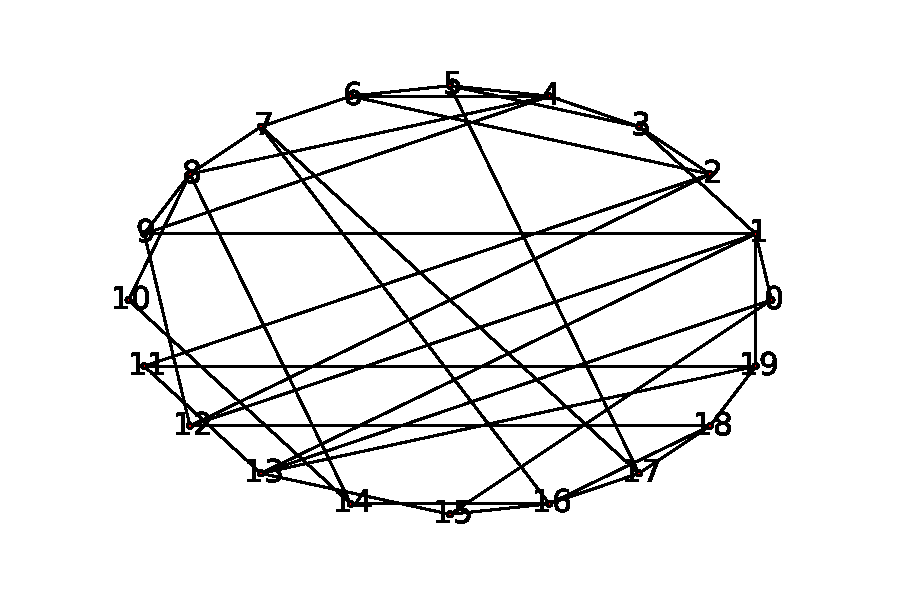
\includegraphics[width=4.2cm, height = 3.0cm]{k4p5-b}}
 \caption{Small World model 3}
 \label{figSW3}
\end{figure}

In Fig. \ref{figSW3}, the network is generated under condition $N=20,K=4,P_{reconnect}=0.5$, the optimal attack strategy given by the algorithm is $\lambda_{8,10}=0.5,\lambda_{14,16}=0.5$, and the optimal result is $P=0.5$. In this topology, node 10's degree is 2, and node 14's degree is 3, they connect to each other. When the attacker obtain the information on edge $(8,10)$ and $(14,16)$, by the result in Remark \ref{exposed condition}, the attacker can perfectly guess the initial information of node 10 and 14. Due to the limited energy of the attacker, when the $\lambda_{8,10} = 0.5,\lambda_{14,16}=0.5$, we can calculate $P_{10}=0.25$ and $P_{14}=0.25$ by Theorem \ref{Them of leakage possibility}. So in the case of under attacks, the degree of privacy leakage in this network is $P = P_{10}+P_{14}=0.5$.

\section{Numerical Examples}\label{Numerical Example}
In this section, we consider a network with 5 nodes as Fig. (\ref{struc}) shows. The real initial state $x^{r}_{i}(0)$ of node 1 to node 5 are set as  $2, 3, 4, 7, 9$, respectively. First, we verify the convergence of the proposed consensus protocol with privacy preserving scheme. As Fig. \ref{uniformDis}, \ref{Gaussian}, \ref{ex} show, all the nodes achieve the average consensus under difference cases. As above mentioned, to hide the initial state of each node, we set the initial state of all the nodes in the algorithm as zero, and hide the information of the initial state of node $i$ in the random offset ${r_{i}(1), r_{i}(2), ..., r_{i}(m_{i})}$, $i=1,\ldots, 5$. Intuitively, the distribution of $r_{i}(k)$ will influence the network performance, such as the convergence rate. Next, we are going to investigate the relation between the convergence rate and the distribution of random offset.
\begin{figure}[!htb]
 \centering
 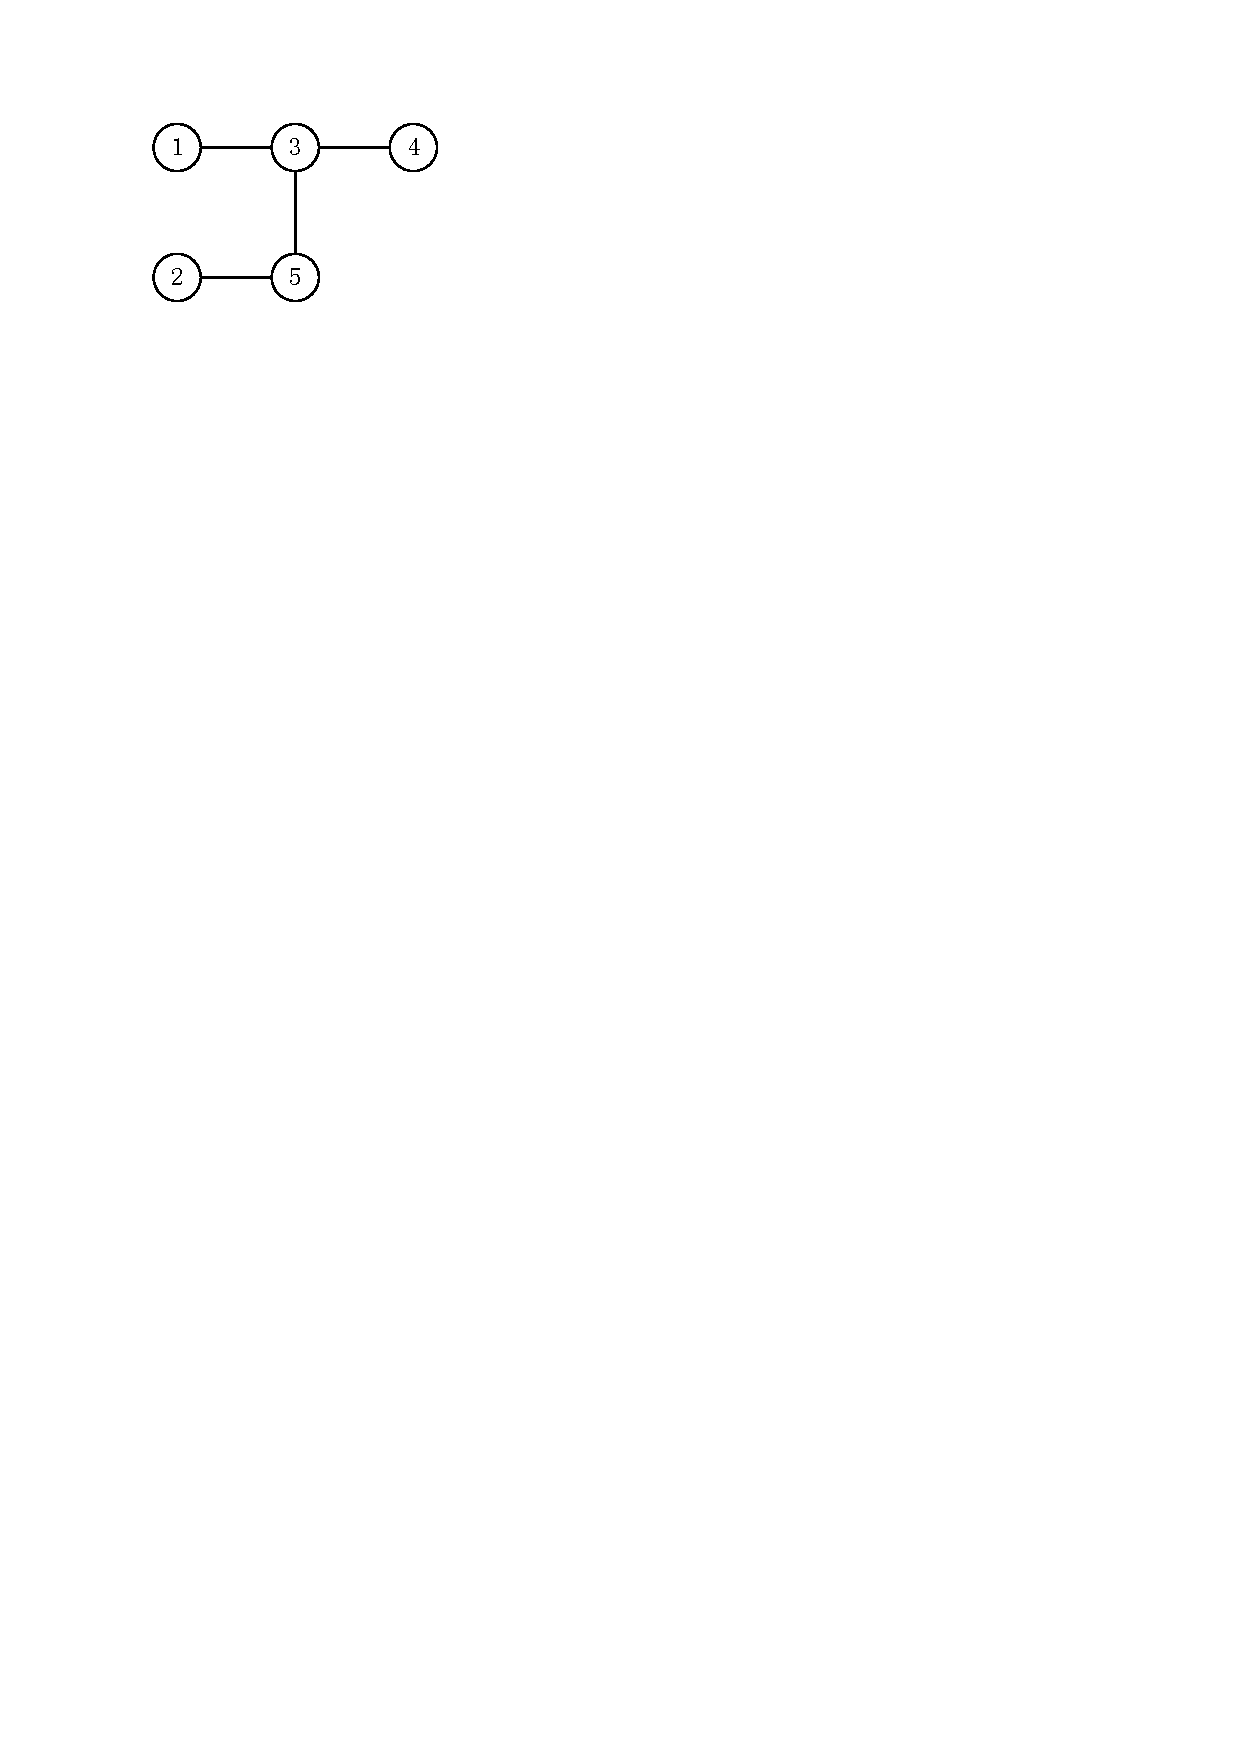
\includegraphics[width=3cm, height=2cm]{structure}
 \caption{Network Structure}
 \label{struc}
\end{figure}
Set $M=20$, and $m_i$ is subject to uniform distribution between $[2,M]$. We simulate the dynamic process of networked system when $r_{i}(k)$ obey uniform, Gaussian and modified exponential distribution, respectively. To make the result can be comparable, we let three kinds of distribution have the same expectation $x_{i}^{r}(0)$, and the length of distribution interval is close to 200. In Gaussian and modified exponential distribution, we require $99.985\%$ random data are in this field. For the given expectation, the distribution interval of standard exponential distribution is fixed. Thus, we need to obtain a modified exponential distribution generated as follow. Firstly, we restrict the length of the standard exponential distribution interval close to 200. Then, we calculate the gap between $x_{i}^{r}(0)$ and the expectation of this distribution. Finally, each random number's value subtract the gap value so that the expectation of this distribution equals to $x_{i}^{r}(0)$. As shown in Fig. \ref{uniformDis}, $r_i(k)$, $i=1,\ldots,5$ satisfies the uniform distribution with its mean equals to the initial state of node $x_{i}^{r}(0)$, and the range of $r_i(k)$ is $[-100+x_{i}^{r}(0),100+x_{i}^{r}(0)]$. Similarly, in Fig. \ref{Gaussian}, $r_{i}(k)$ satisfies the gaussian distribution with $r_i(k)\thicksim N(x_{i}^{r}(0),1000)$. In Fig. \ref{ex}, $r_{i}(k)$ is subject to the modified exponential distribution with expectation $x_{i}^{r}(0)$ and variance 992.25.

\begin{figure}[!htb]
 \centering
 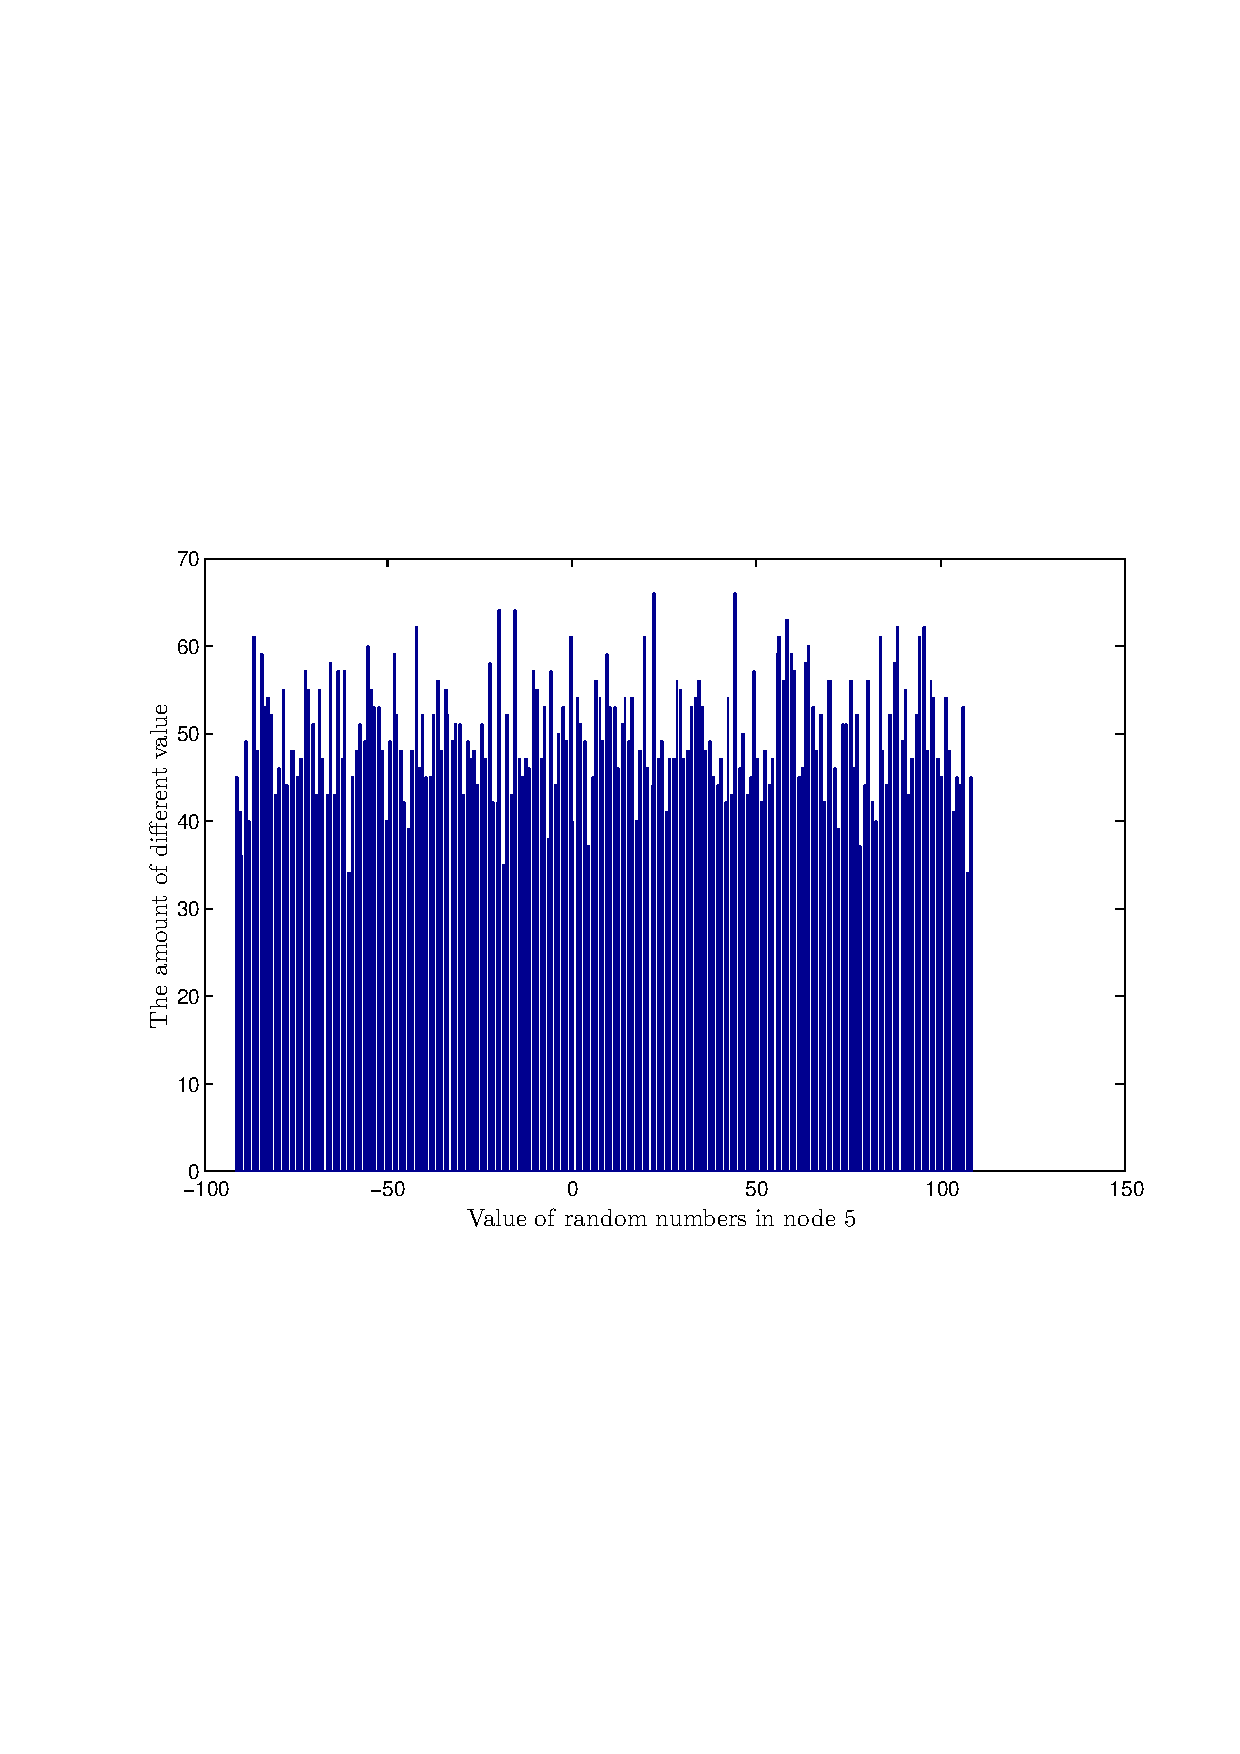
\includegraphics[width=3.3cm, height=2.6cm]{NMDis}
 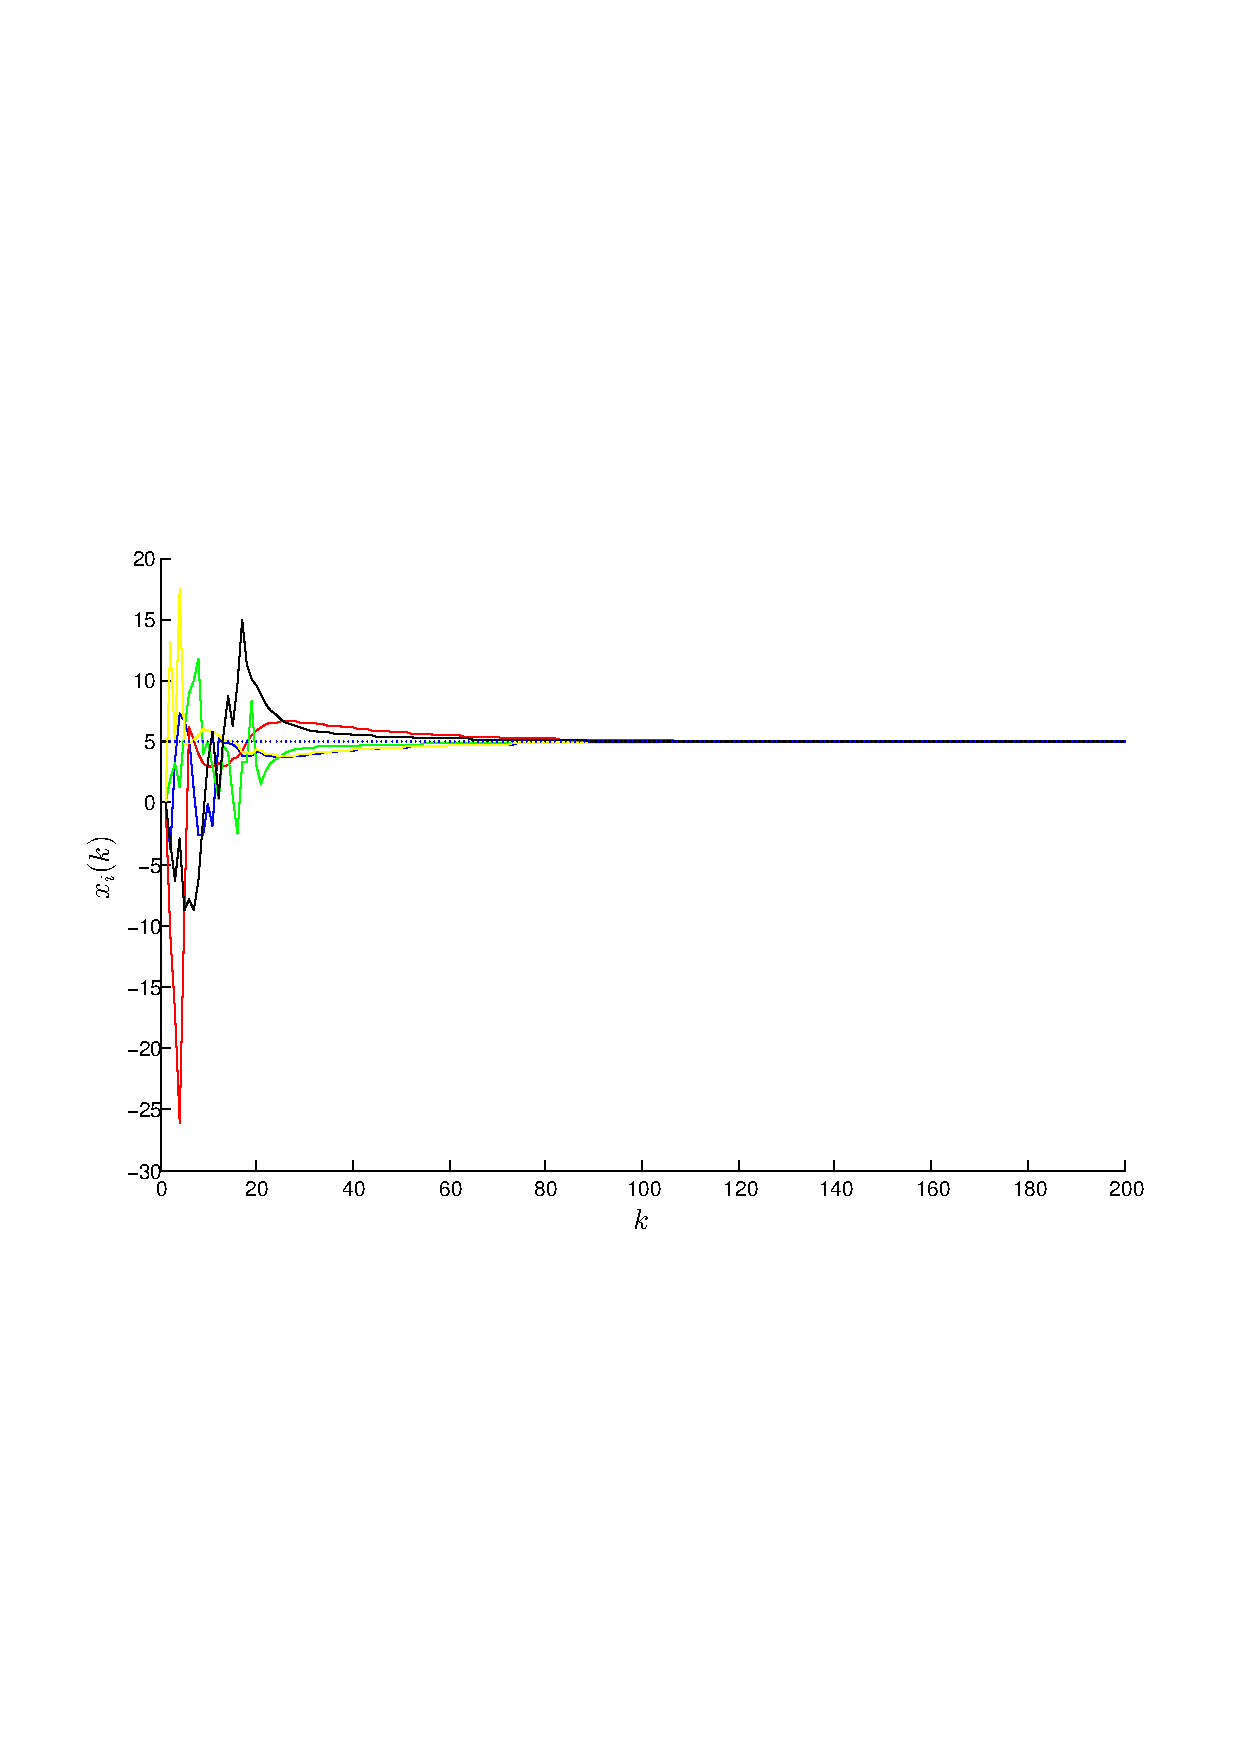
\includegraphics[width=3.3cm, height=2.6cm]{Normconsensus}
 % \subcaption{Norm}
 %\label{normconsensus}
 \caption{Uniform distribution and consensus process}\label{uniformDis}
\end{figure}

\begin{figure}[!htb]
 \centering
 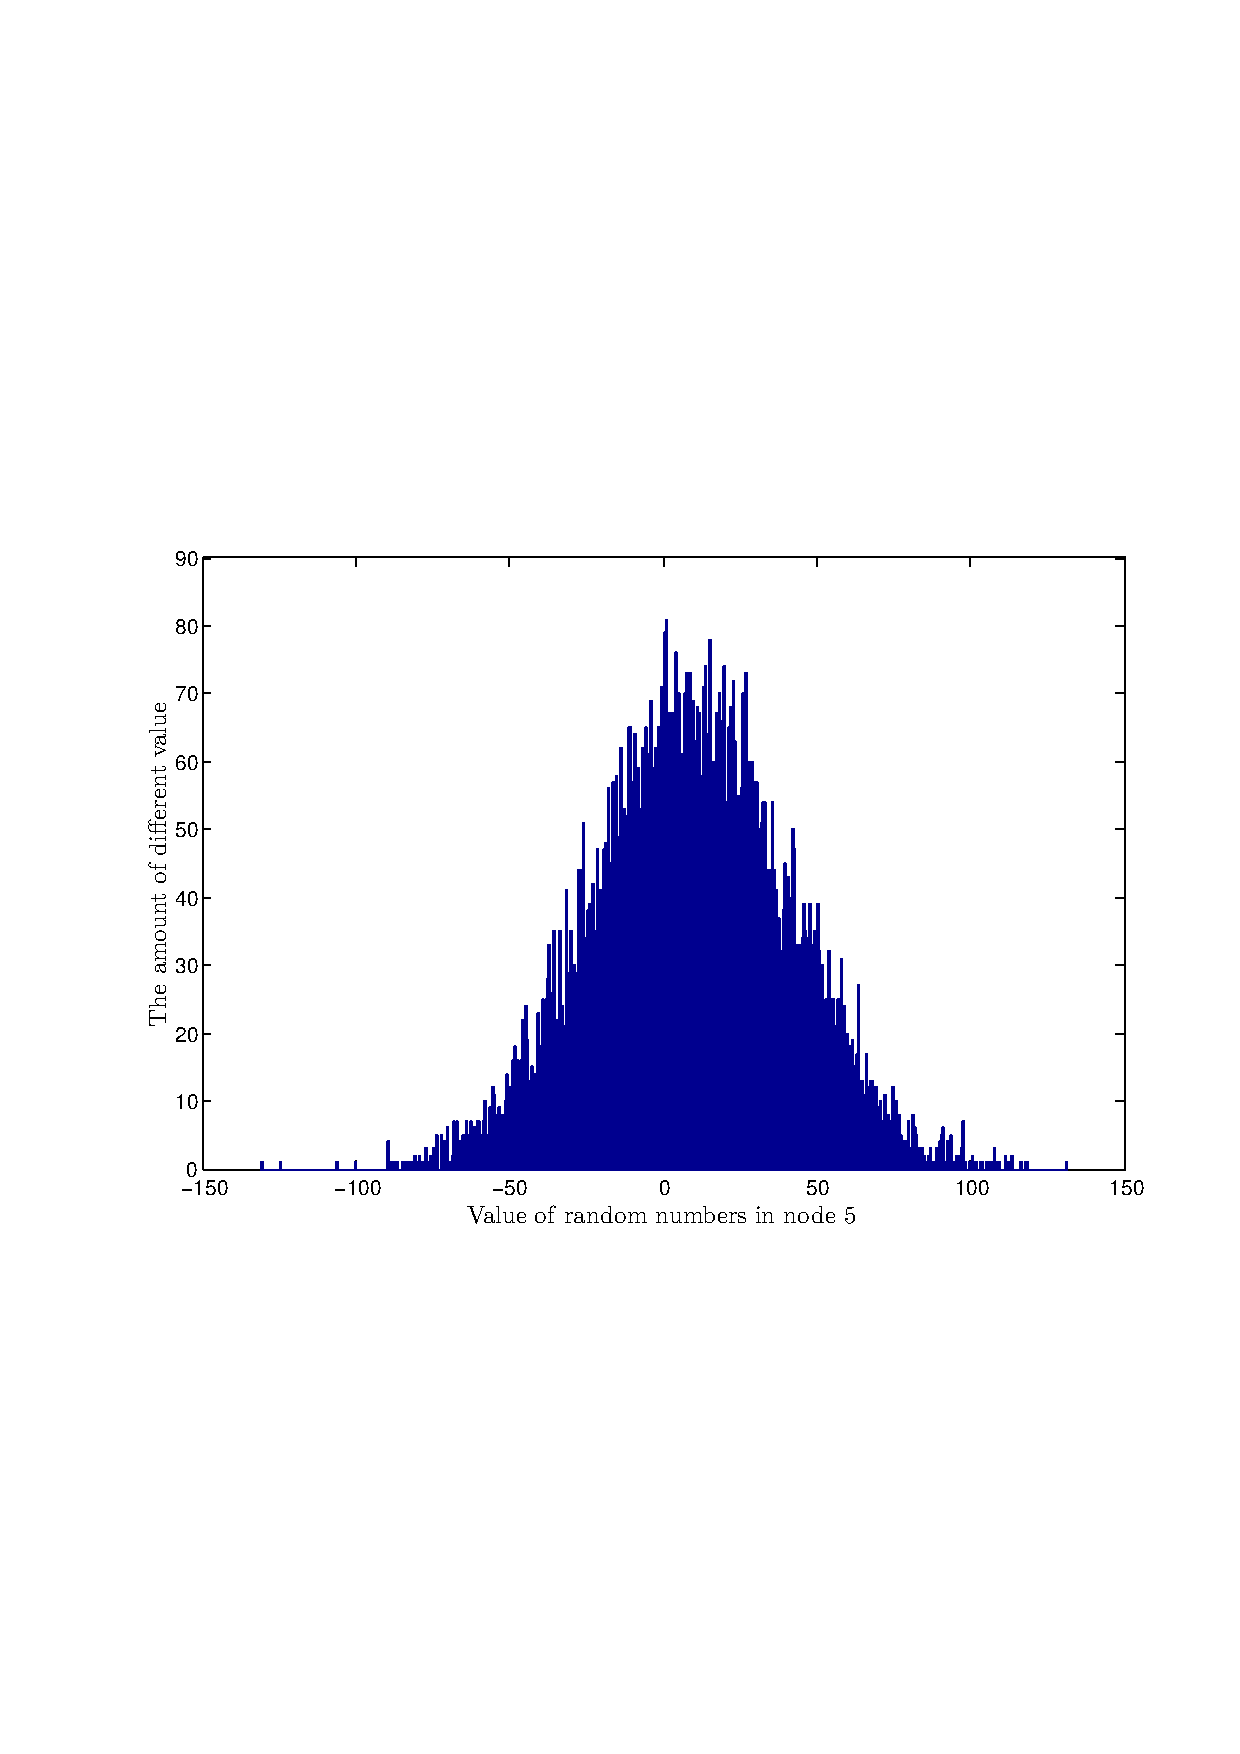
\includegraphics[width=3.3cm, height=2.6cm]{GSDis}
 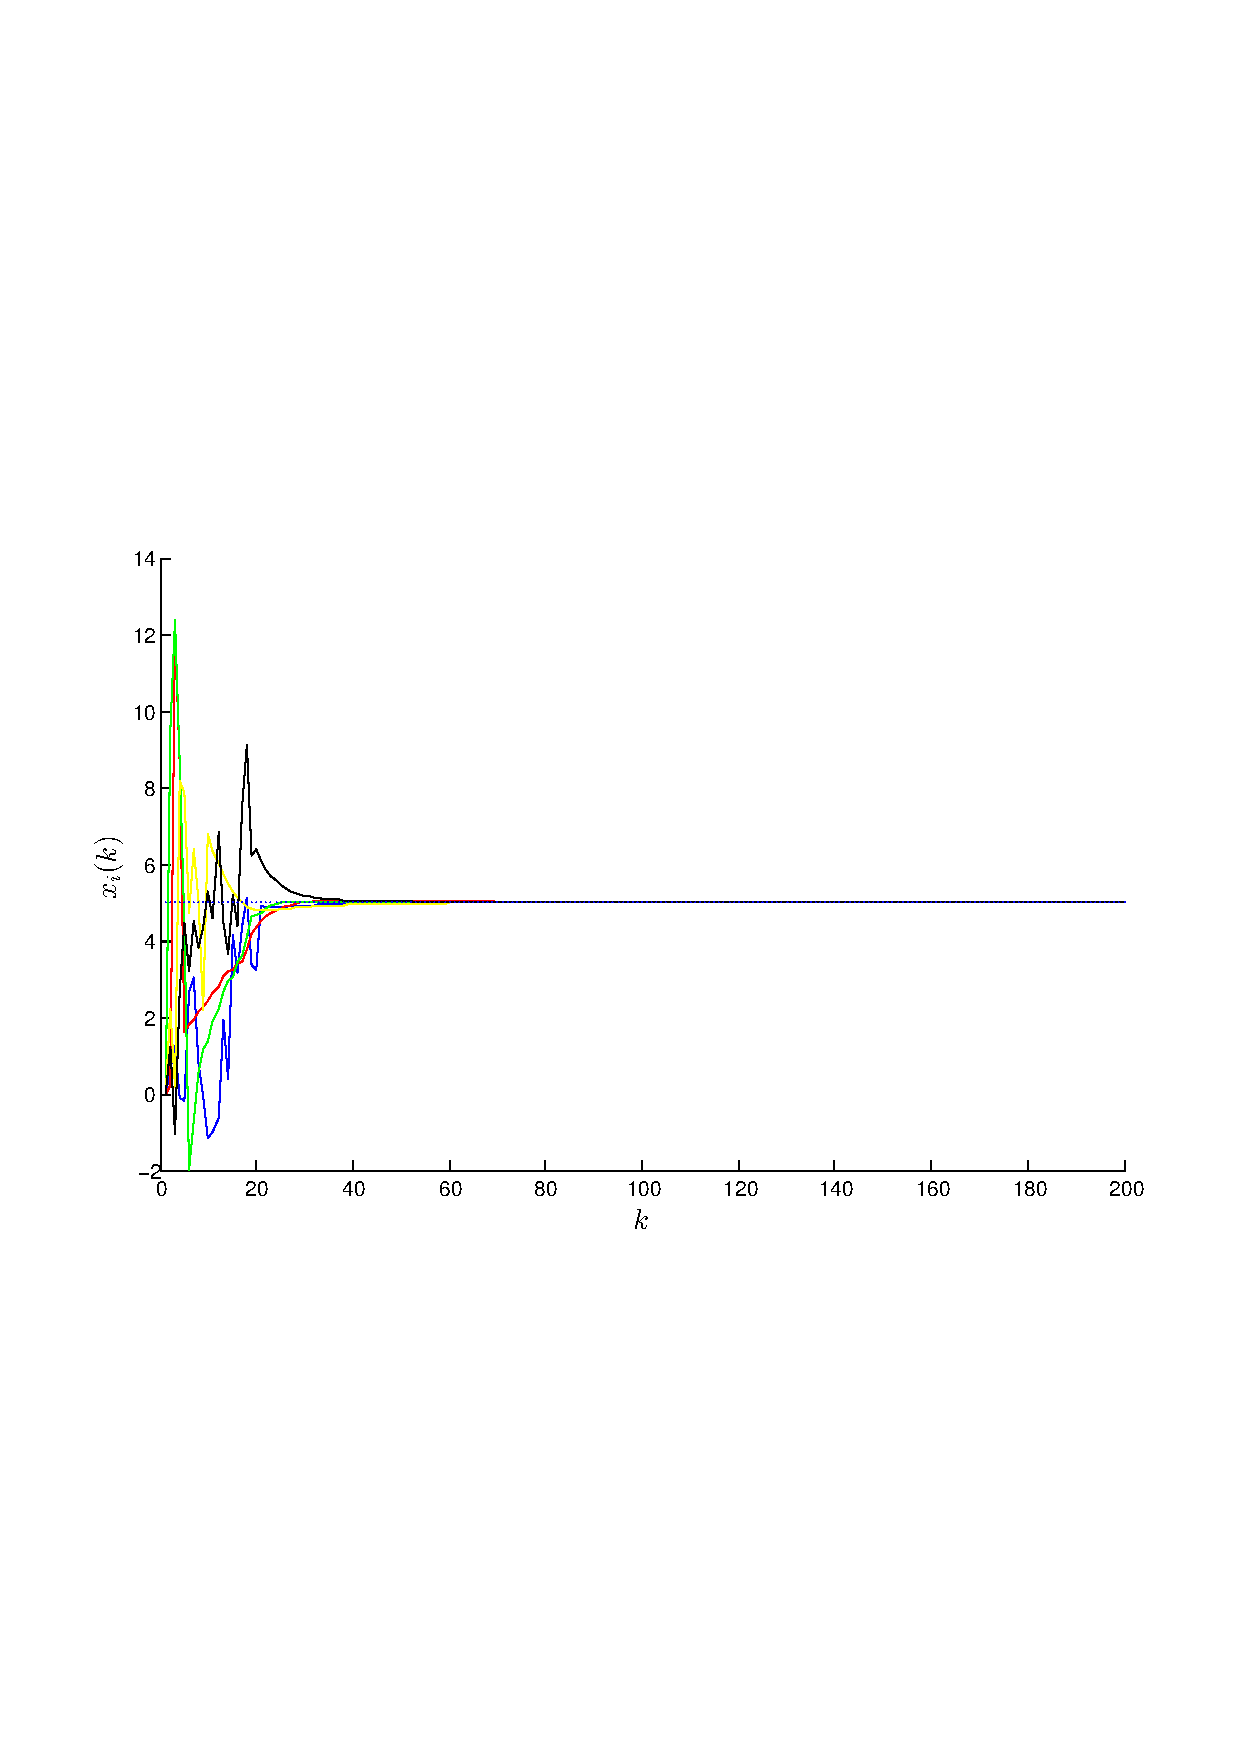
\includegraphics[width=3.3cm, height=2.6cm]{GSconsensus}
 % \subcaption{Norm}
 %\label{normconsensus}
 \caption{Gaussian distribution and consensus process}\label{Gaussian}
\end{figure}

\begin{figure}[!htb]
 \centering
 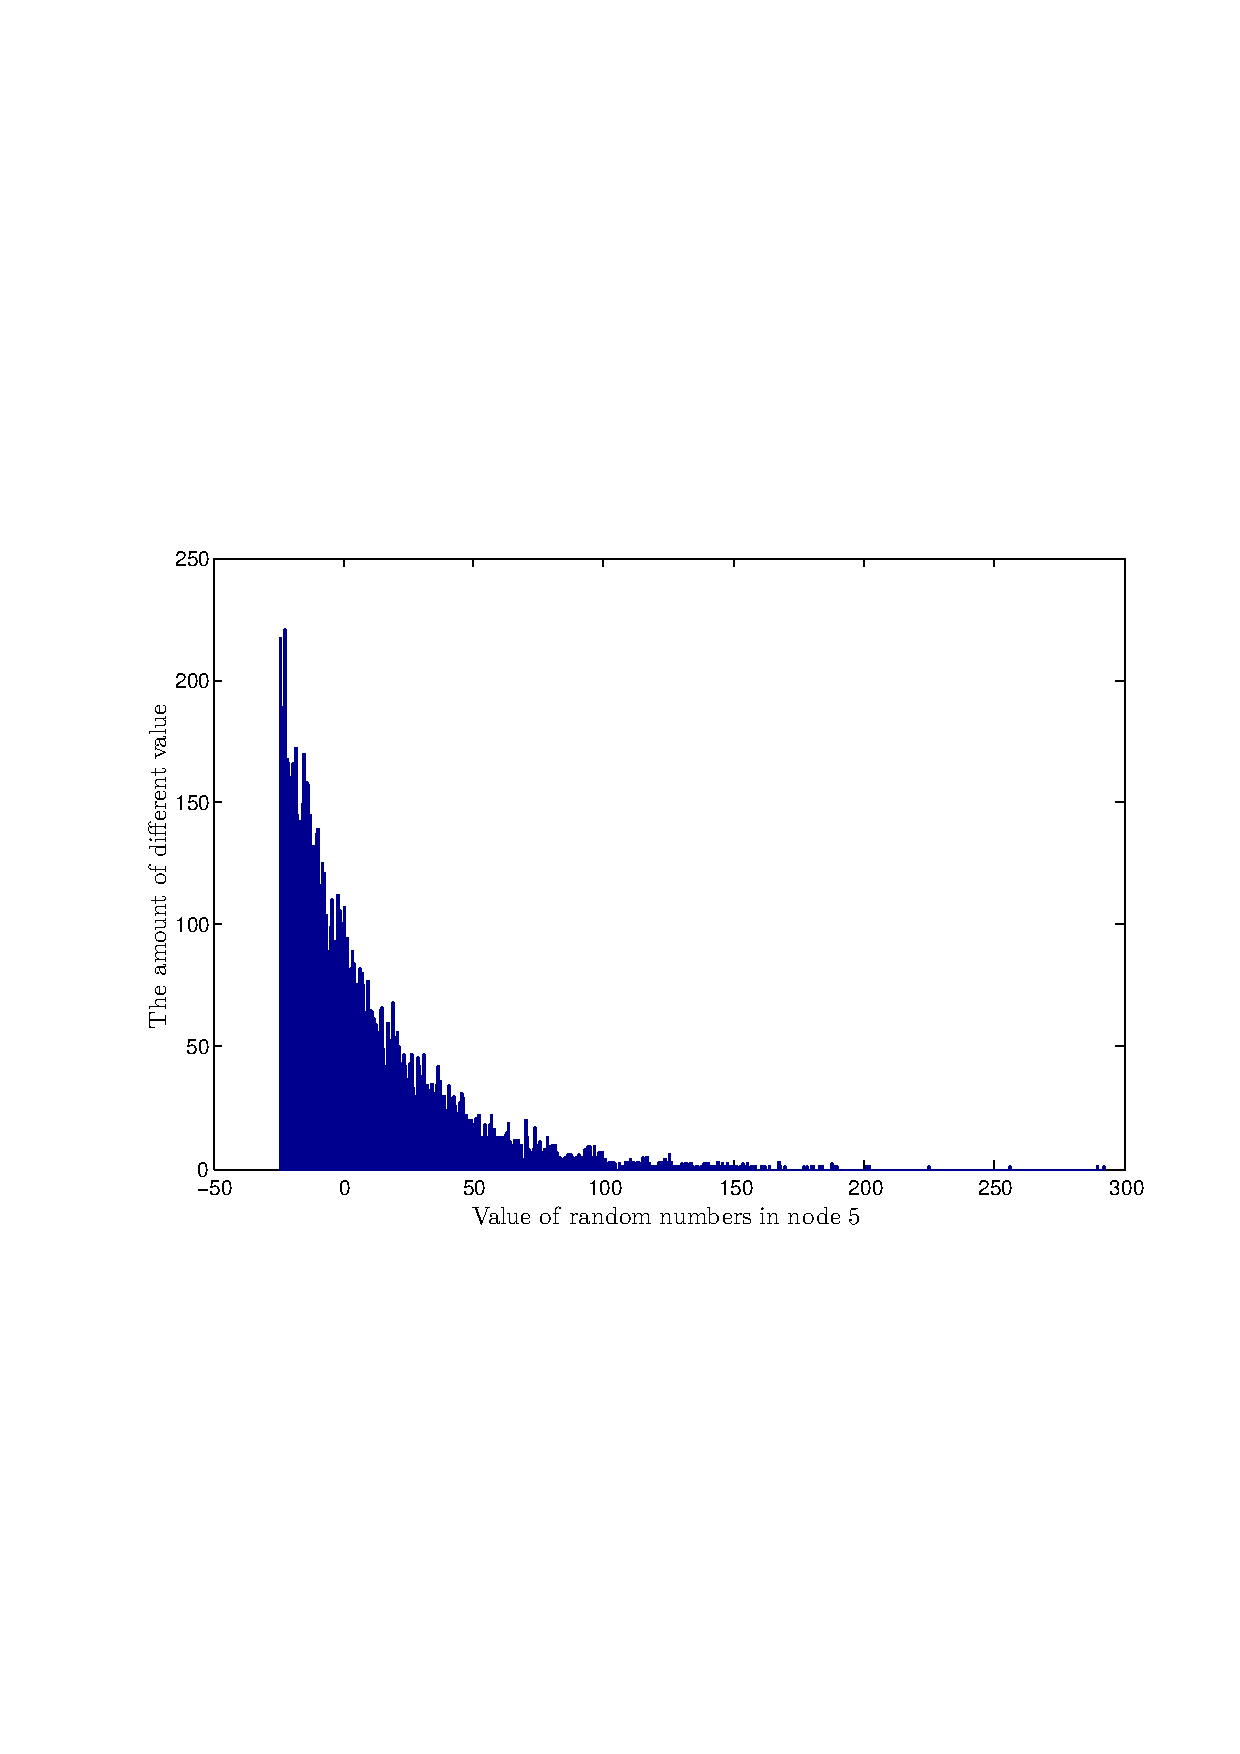
\includegraphics[width=3.3cm, height=2.6cm]{EXDis}
 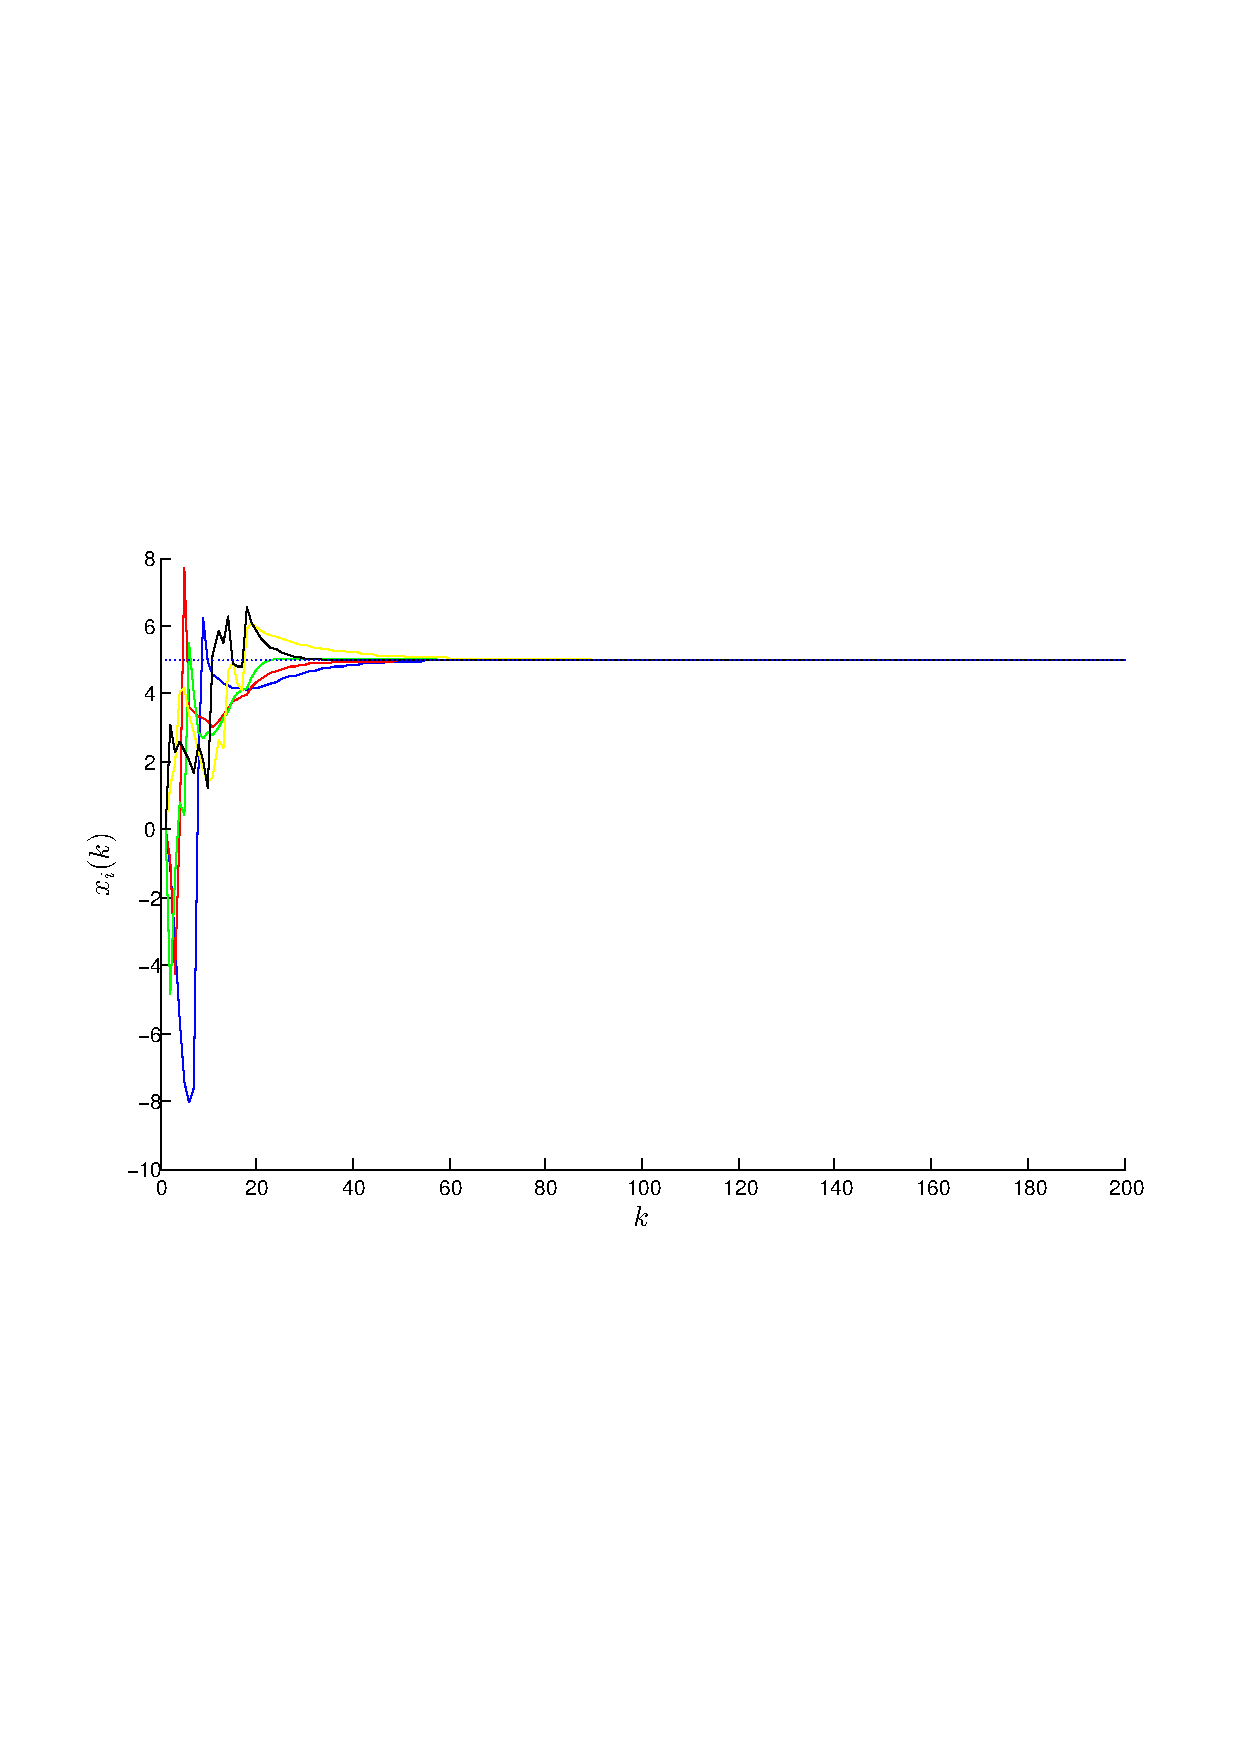
\includegraphics[width=3.3cm, height=2.6cm]{EXconsensus}
 \caption{Modified exponential distribution and consensus process}\label{ex}
\end{figure}

Here, similar to the definition of settling time in classical control theory, we set the convergence time of reaching average consensus as the time at which the average states of all the nodes enters into $[4.9,5.1]$. For different distribution of $r_i(k)$, all the simulations are averaged by 2000 times, and the results are listed in Table \ref{convergence step}. Obviously, all the nodes converge to the mean of the initial states despite of different distribution of $r_i(k)$. However, the convergence time is totally different. As we can see, the uniform distribution case leads to the maximum convergence time when compared with the other two cases, and the time in case of Gaussian and modified exponential distribution is same. Then, we calculate the variance in above distributions as 3333.33, 1000 and 992.25, the latter two are closer. To verify the the influence of variance of distribution, we add a case that $r_{i}(k)$ subject to uniform distribution between $[-55+x_{i}^{r}(0),55+x_{i}^{r}(0)]$, i.e., the variance is 1008.33, then we can obtain the convergence time 61. Thereby, despite of the difference between distribution form, convergence time is only related to the variance of distribution.

\begin{figure}[!htb]
\centering
\begin{tabular}{cccc}
Distribution & Convergence steps \\\hline
Uniform & 70\\ \hline
Gaussian  &61 \\ \hline
Modified exponential &61 \\ \hline
\end{tabular}
\captionsetup{type=table}
\caption{Convergence step}\label{convergence step}
\end{figure}


\section{Conclusion} \label{Conclusion}
In this paper, we have studied the attack problem in the network with privacy protection. We have shown an proposed privacy preserving algorithm, where each node add well-designed noise while update their value in the process of consensus, and there is a defect in the algorithm, when the network topology satisfied an specific condition, the privacy leakage problem will occur. While there is an attacker in the network can intercept the data transmitted on the edges, we have derived the probability of network disclosure. For the attacker with limited energy, we have further found the optimal attacking strategy in ring network and small-world model. Combined with an optimization algorithm, we give some guiding suggestion to find the optimal attack strategy. From the simulation results, we get the conclusion that the variance of the adding noise's distribution will influence the convergence time of the privacy preserving consensus protocol.

\appendices
\section{Proof of the First Zonklar Equation}
Appendix one text goes here.

% you can choose not to have a title for an appendix
% if you want by leaving the argument blank
\section{}
Appendix two text goes here.


% use section* for acknowledgment
\ifCLASSOPTIONcompsoc
  % The Computer Society usually uses the plural form
  \section*{Acknowledgments}
\else
  % regular IEEE prefers the singular form
  \section*{Acknowledgment}
\fi


The authors would like to thank...


% Can use something like this to put references on a page
% by themselves when using endfloat and the captionsoff option.
\ifCLASSOPTIONcaptionsoff
  \newpage
\fi


\bibliographystyle{unsrt}
\bibliography{ieeeconf}


\begin{IEEEbiography}{Michael Shell}
Biography text here.
\end{IEEEbiography}

% if you will not have a photo at all:
\begin{IEEEbiographynophoto}{John Doe}
Biography text here.
\end{IEEEbiographynophoto}

% insert where needed to balance the two columns on the last page with
% biographies
%\newpage

\begin{IEEEbiographynophoto}{Jane Doe}
Biography text here.
\end{IEEEbiographynophoto}


\end{document}


